\documentclass[11pt,a4paper,oneside]{book}
\newcommand{\NumeroRelazione}{5}

\newcommand{\TitoloRelazione}{Misure di riflessione nei risonatori}
\usepackage[utf8]{inputenc}       
\usepackage[T1]{fontenc}          
\usepackage[italian]{babel}       
\usepackage{graphicx}             
\usepackage{float}
\usepackage{amsmath}
\usepackage{amsfonts} 
\usepackage{amssymb}  
\usepackage{steinmetz}
\usepackage{pgfplots}
\usepackage{tikz}
\usepackage{enumitem} 
\usepackage{subcaption}
\usepackage{caption}
\usepackage{comment}
\usepackage[normalem]{ulem}
\usepackage[americaninductors, siunitx]{circuitikz}

\usetikzlibrary{arrows.meta, patterns, shapes.geometric, calc, positioning, shapes, arrows}
\pgfplotsset{compat=1.18}

% --- GEOMETRY (Margini e distanze) ---
\usepackage[
    a4paper,
    top=3.5cm,      
    bottom=3cm,    
    left=3cm,      
    right=3cm,     
    headheight=40pt, % Spazio per l'immagine
    headsep=25pt     % Distanza tra immagine e testo/titoli
]{geometry}

% --- FANCYHDR (Intestazioni) ---
\usepackage{fancyhdr} 
\pagestyle{fancy}
\fancyhf{} 
\fancyhead[L]{
\includegraphics[height=1cm]{Images/top.png}} 
\fancyhead[R]{\thepage} 
\fancyhead[C]{\textit{\leftmark}} 

% Per avere l'intestazione anche nelle pagine iniziali dei capitoli
\fancypagestyle{plain}{
  \fancyhf{}
  \fancyhead[L]{
\includegraphics[height=1cm]{Images/top.png}}
  \fancyhead[R]{\thepage}
  \fancyhead[C]{\textit{\leftmark}}
  \renewcommand{\headrulewidth}{0.4pt}
}

% --- LINK CLICCABILI (Senza il backtick d'errore) ---
\usepackage[hidelinks]{hyperref} 
 

% --- COMANDI PERSONALIZZATI ---
\newcommand{\tikznode}[2]{%
  \ifmmode%
    \tikz[remember picture,baseline=(#1.base),inner sep=0pt] \node (#1) {$#2$};%
  \else
    \tikz[remember picture,baseline=(#1.base),inner sep=0pt] \node (#1) {#2};%
  \fi%
}
\tikzset{portnode/.style={circle, draw, inner sep=1pt, font=\scriptsize}}


\begin{document}
% --- PAGINA DEL TITOLO 
\begin{titlepage}
    \centering
    {\scshape\Large Università degli Studi "La Sapienza" \par} 
    \vspace{0.5cm}
    {\scshape\large Dipartimento di Ingegneria dell'Informazione, Elettronica e Telecomunicazioni \par}
    \vspace{0.5cm}
    {\scshape\large Corso di Laurea in Ingegneria Elettronica \par}
    \vspace{1.5cm}
    {\huge\bfseries Laboratorio Multidisciplinare\\ di Elettronica I\par}
    \vspace{0.35cm}
    {\Large\bfseries Relazione \NumeroRelazione\par}
    \vspace{0.35cm}
    {\Large\bfseries \TitoloRelazione\par}
    \vspace{1cm}
    {\large CFU:  6 \par} 
    \vspace{2.5cm}

    {\large Gruppo 18: \par}
    \vspace{0.2cm}
    {\Large Renato Bearzotti \par}
    {\Large Nicolò Falasca \par}

    \vspace{0.8cm}
    \IfFileExists{Images/top.png}{%
        
\includegraphics[width=3.5cm]{Images/top.png}\par
    }{}
    \vspace{0.35cm}
    \IfFileExists{Images/logo Sapienza (rgb).png}{%
        
\includegraphics[width=6.8cm]{Images/logo Sapienza (rgb).png}\par
    }{}
    \vspace{0.8cm}

    % Professori allineati a destra
    \begin{minipage}[t]{\textwidth}
        \begin{flushright}
            \large
            \textbf{Professori:}\\
            Andrea Mostacci\\
            Stefano Pisa\\
            Pasquale Tommasino
        \end{flushright}
    \end{minipage}

    \vfill
    {\large Anno Accademico 2026-2027 \par}
\end{titlepage}


\frontmatter 
\tableofcontents

\mainmatter
 
 
\chapter{Deflettore RF (banda S): identificazione dei modi}
Lo scopo dell'esercitazione è misurare due cavità risonanti, lavoranti a frequenze diverse, e valutarne i vari parametri
caratteristici.
\\Il primo deflector è progettato per lavorare a 2.856GHz (banda-S).
\\Per prima cosa abbiamo identificato i modi del delfettore eccitato da un'antenna, misurando tra 1.5GHz e 3GHz (restando nei limit della calibraizone).
\\Il risultato è il seguente grafico.
\begin{figure} [H]
    \centering
    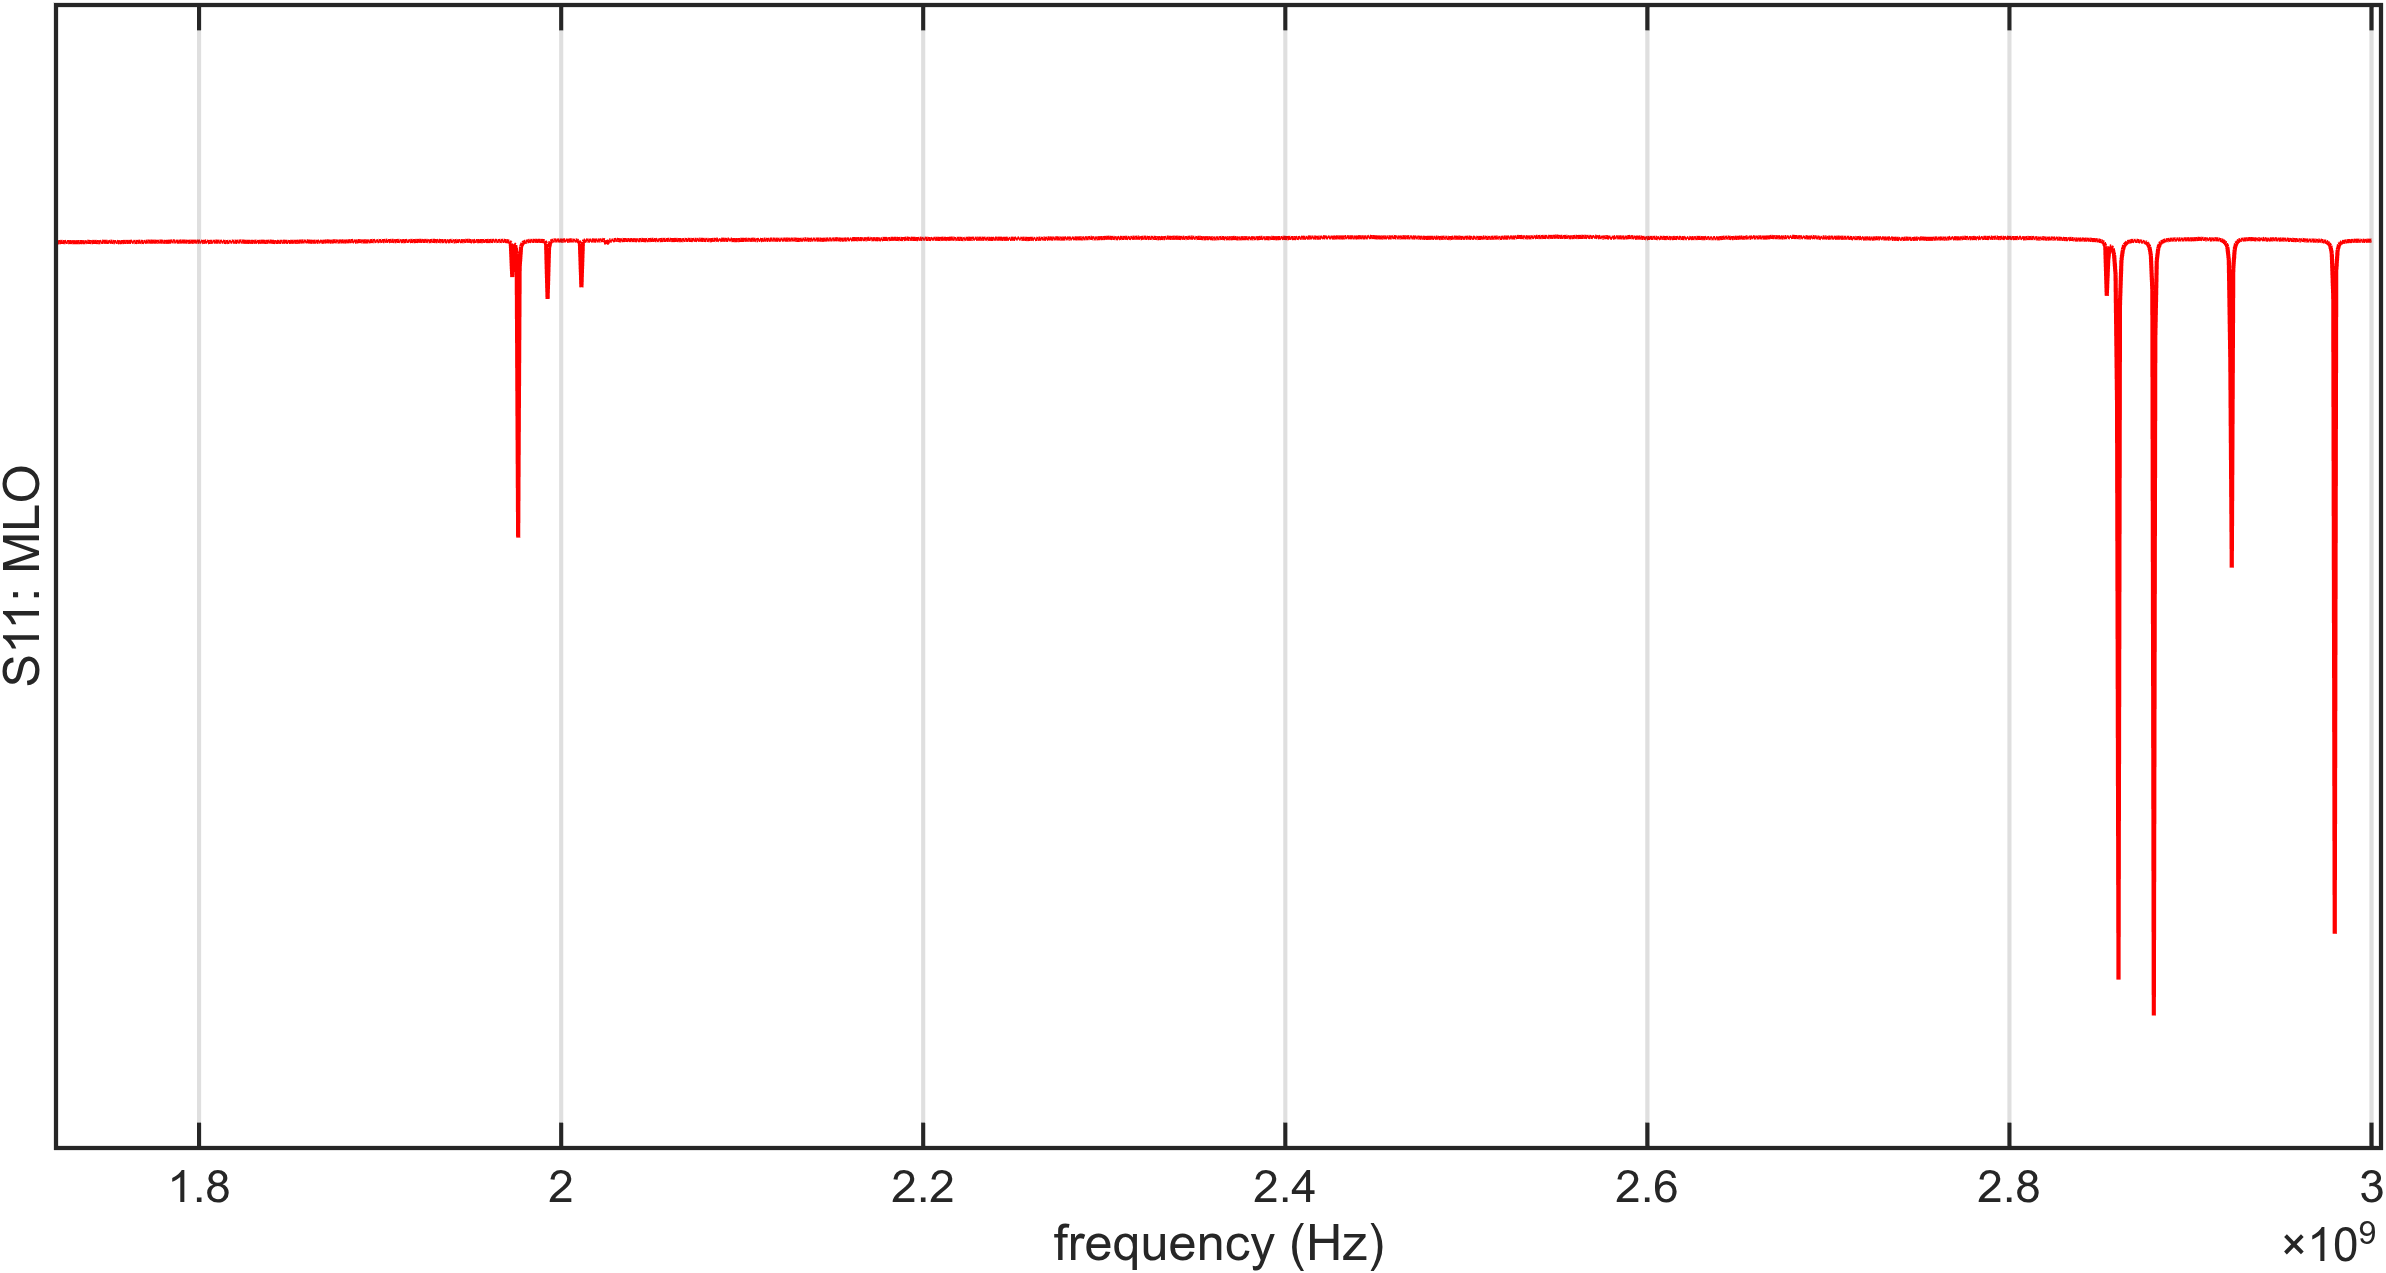
\includegraphics[width=0.6\textwidth]{./Images/Relazione5_Foto/1_1_modi_generali.png}
    \caption{Misura della frequenza di risonanza dei modi fino a 3GHz eccitati dall'antenna.}
\end{figure} 
Come si nota di modi sono divisi in due gruppi, ognuno dei quali corrisponde al modo di una singola cella risonante del delfettore.
\\Di seguito uno zoom sui due range dove troviamo i picchi.
\begin{figure}[H]
    \centering
    \begin{minipage}[t]{0.45\textwidth}
        \centering
        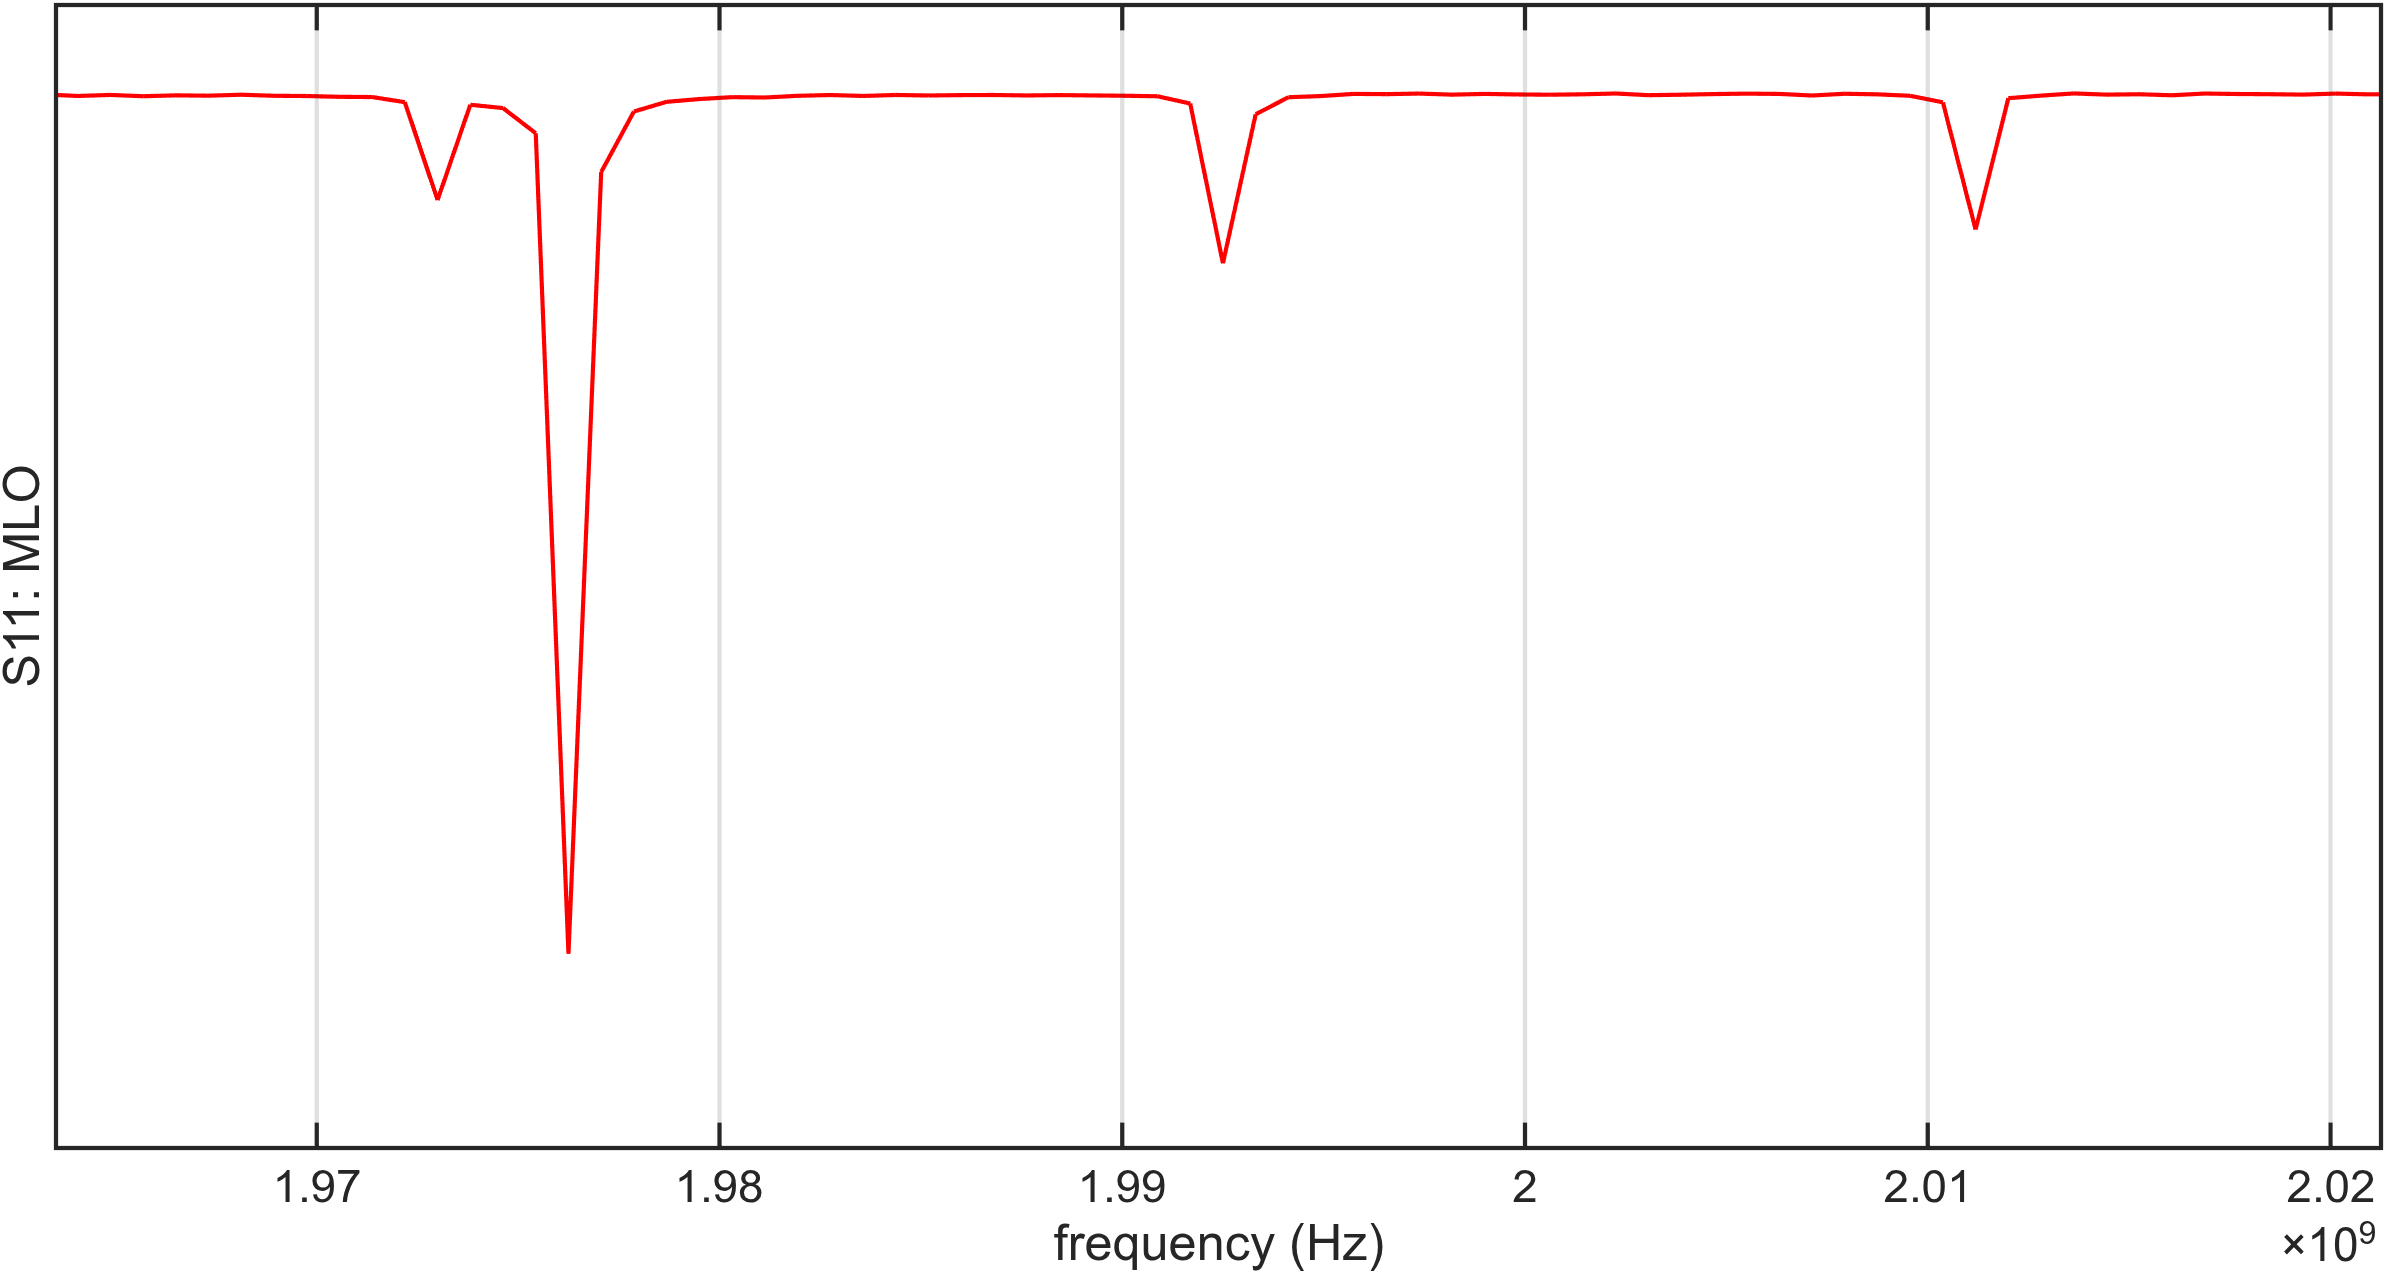
\includegraphics[width=0.9\textwidth]{./Images/Relazione5_Foto/1_2_zoom_sx.png}
        \caption{Risonanza dei modi tra 1.965 e 2.02 GHz.}
    \end{minipage}
    \hfill
    \begin{minipage}[t]{0.45\textwidth}
        \centering
        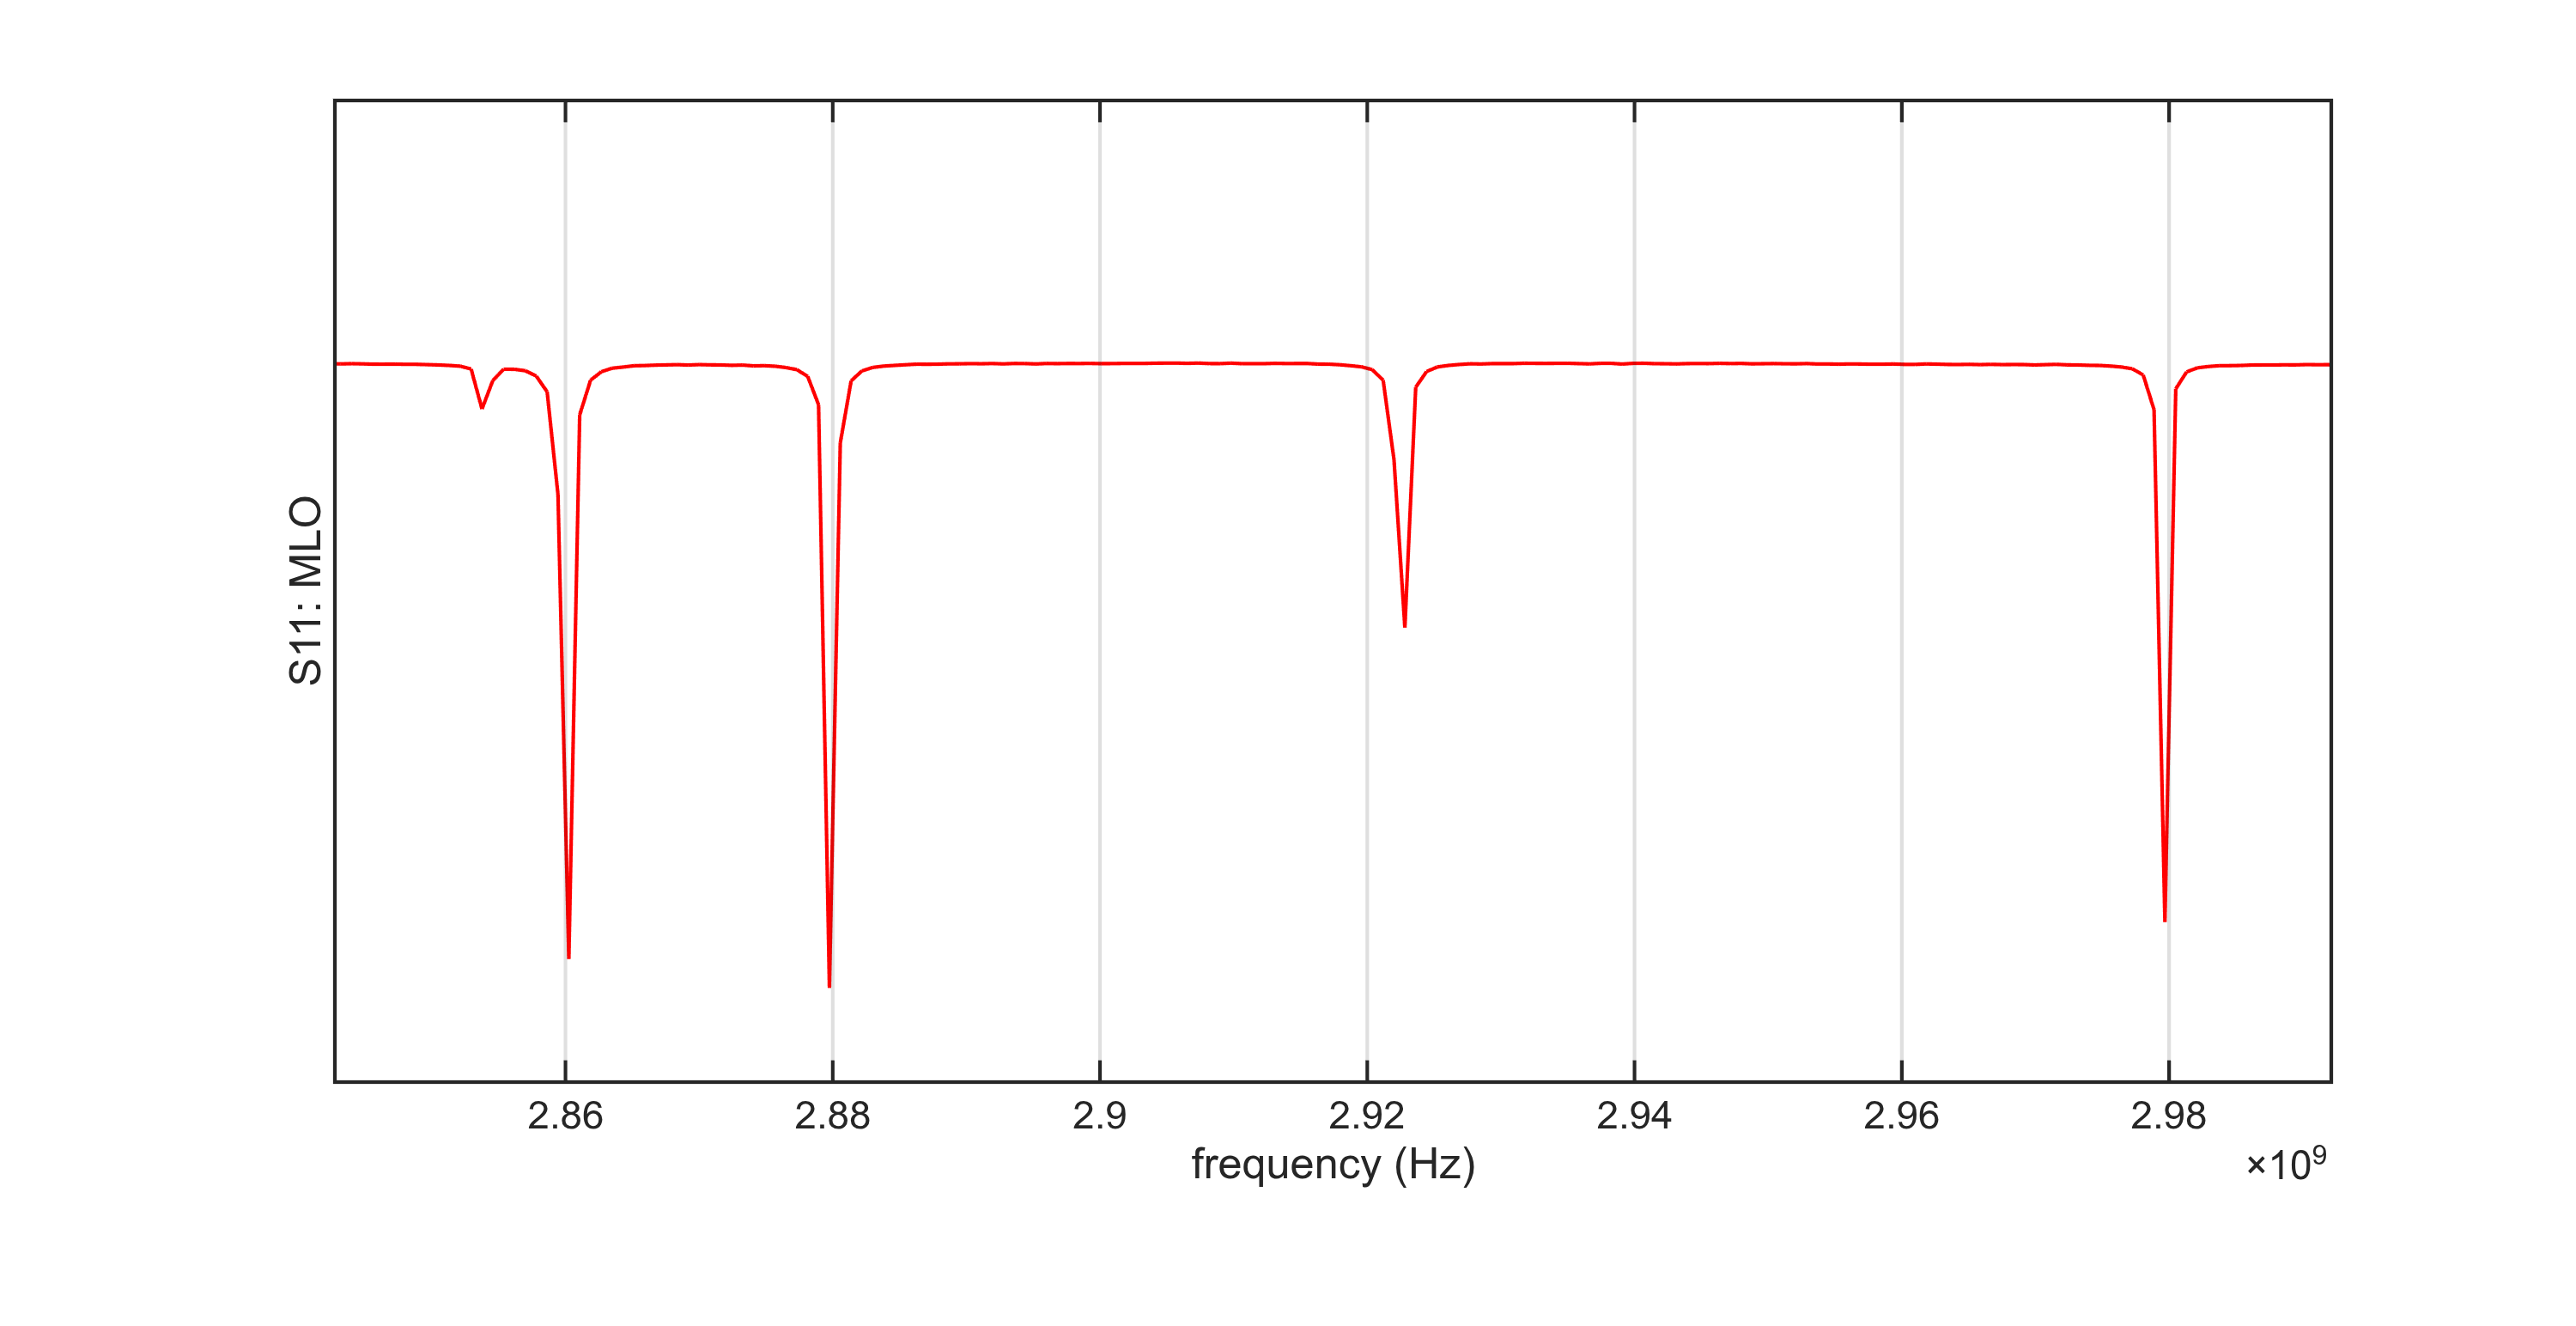
\includegraphics[width=\textwidth]{./Images/Relazione5_Foto/1_3_zoom_dx.png}
        \caption{Risonanza dei modi tra 2.85 e 2.99 GHz.}
    \end{minipage}
\end{figure}
Come si nota facilmente il primo gruppo di modi è a circa 1.976GHz, mentre il secondo è a circa 2.860GHz.
\\Come si vede chiaramente dai due grafici il valore di $|S_{11}|_{dB}$ è inferiore nel secondo range di frequenze, ed infatti il delfettore lavora a 2.856GHz proprio per questo motivo.


\chapter{Deflettore RF (banda S): modi di tipo TM$_{010}$}
\section{Misura della frequenza di risonanza, del fattore di qualità unloaded, $Q_0$, e del coefficiente di accoppiamento $\beta$}
\subsection{Misura della frequenza di risonanza}
Ci siamo centrati nel primo gruppo di modi risonanti ed in particolare abbiamo preso il modo con il valore di $|S_{11}|$ inferiore e abbiamo centrato lo span intorno alla sua frequenza.
\\Il grafico è:
\begin{figure}[H]
    \centering
    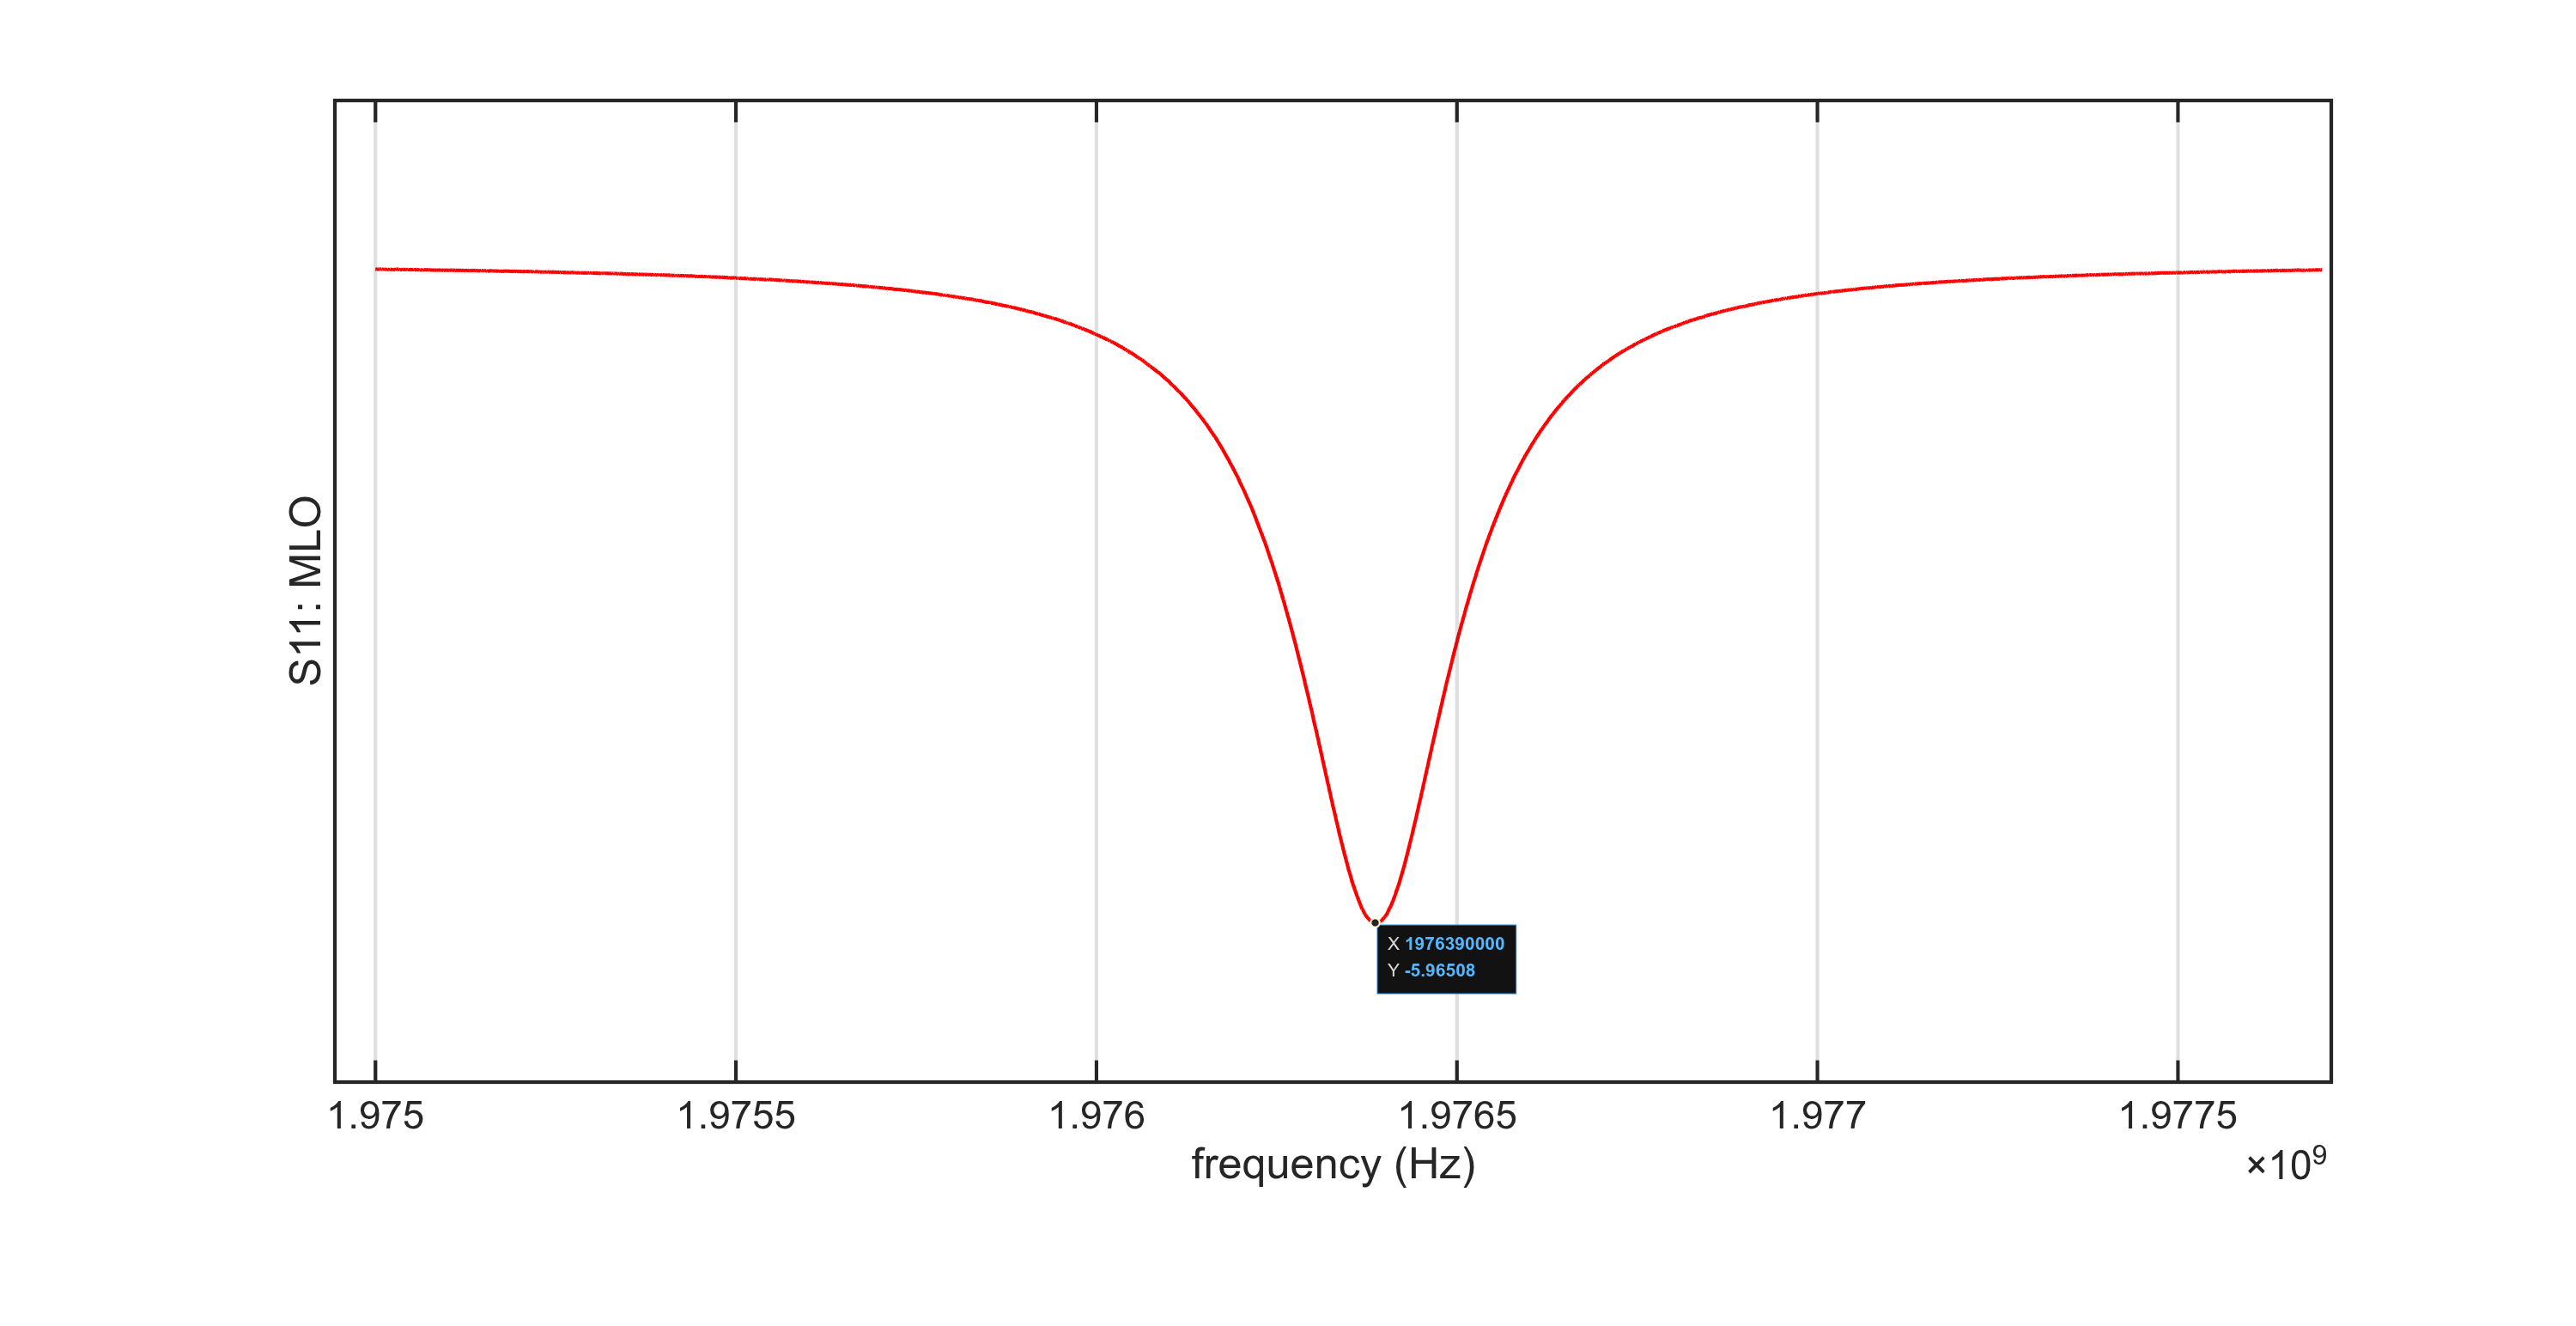
\includegraphics[width=0.6\textwidth]{./Images/Relazione5_Foto/2_1_misura_f0.png}
    \caption{Misura della frequenza di risonanza e del modo con $|S_{11}|_{dB}$ minore nel primo gruppo di modi.}
\end{figure}
Da lui ricaviamo:
\begin{equation}
    f_0=1.97637 \quad GHz
\end{equation}
\subsection{Misura del fattore di qualità unloaded, $Q_0$}
Di seguito vediamo i vari passaggi per misurare il fattore di qualità unloaded, $Q_0$, e il coefficiente di accoppiamento $\beta$.
Per prima cosa abbiamo misurato $S_{11}$ e lo abbiamo graficato sullo Smith chart. Il risultato è il seguente .
\begin{figure}[H]
    \centering
    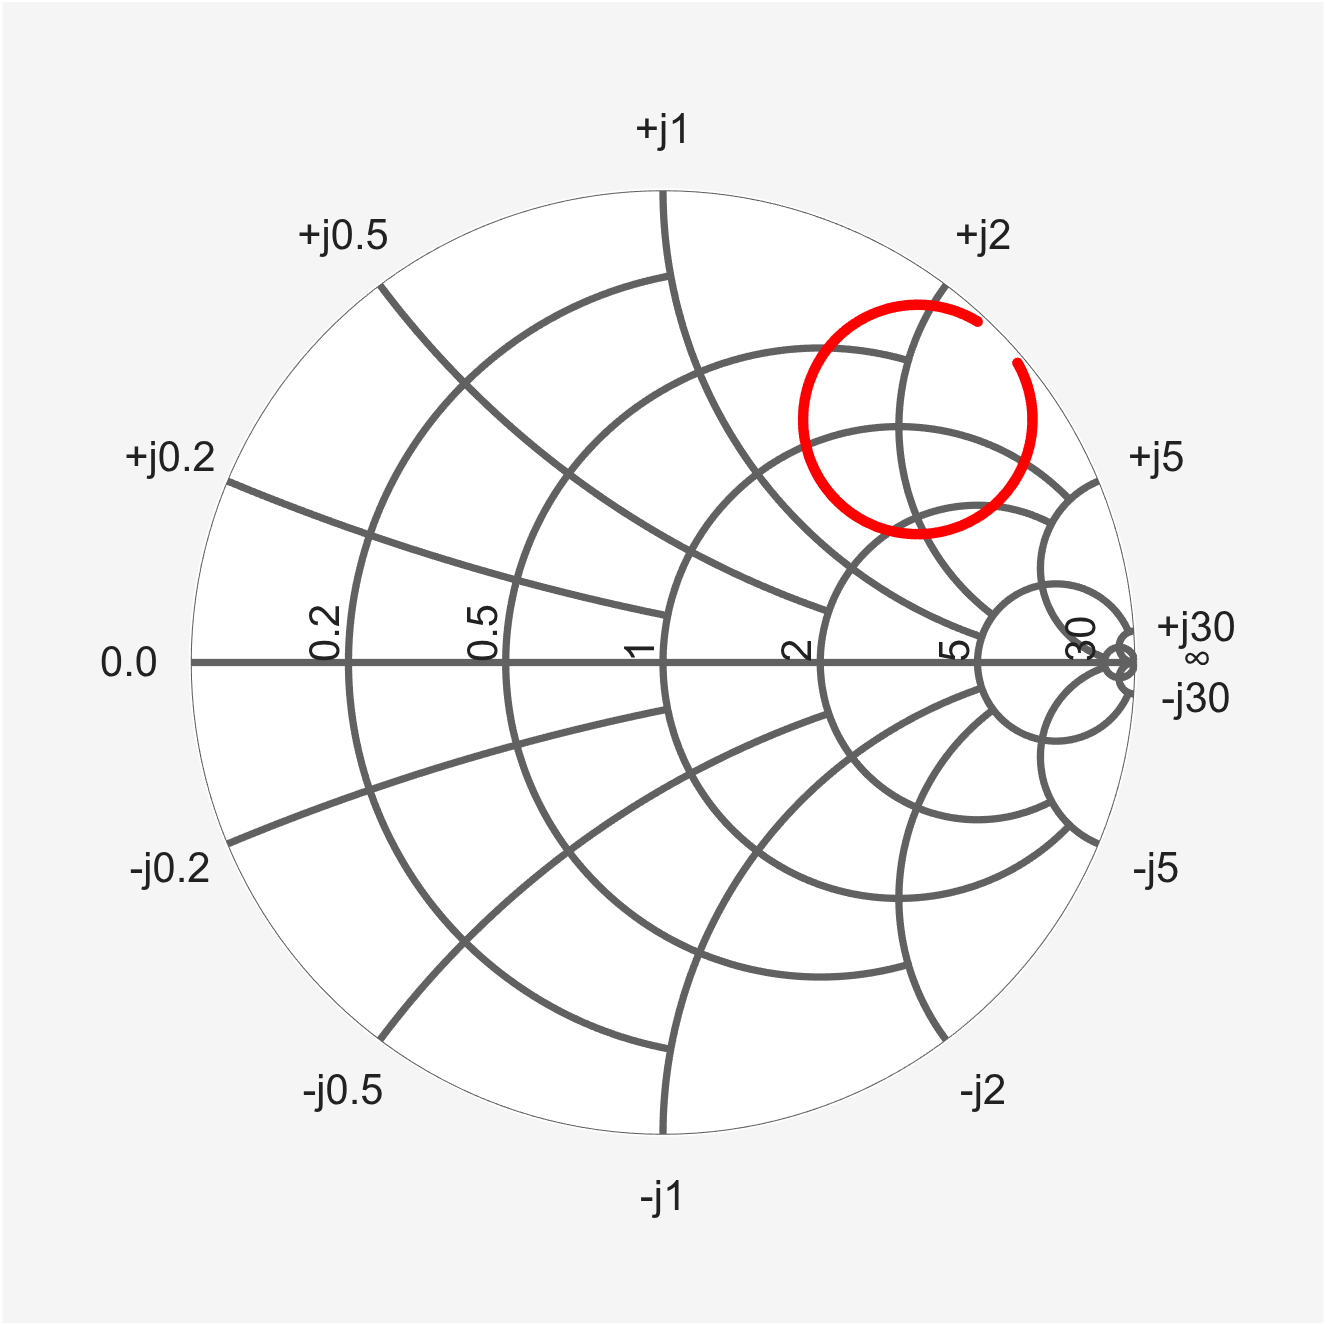
\includegraphics[width=0.3\textwidth]{./Images/Relazione5_Foto/2_2_fase_smith_chart_non_modificata.png}
    \caption{Misura di $S_{11}$ sullo Smith chart.}
\end{figure}
Poi abbiamo introdotto un offset di fase di 43.52° per portare lo Smith chart in posizione di open position.
\begin{figure}[H]
    \centering
    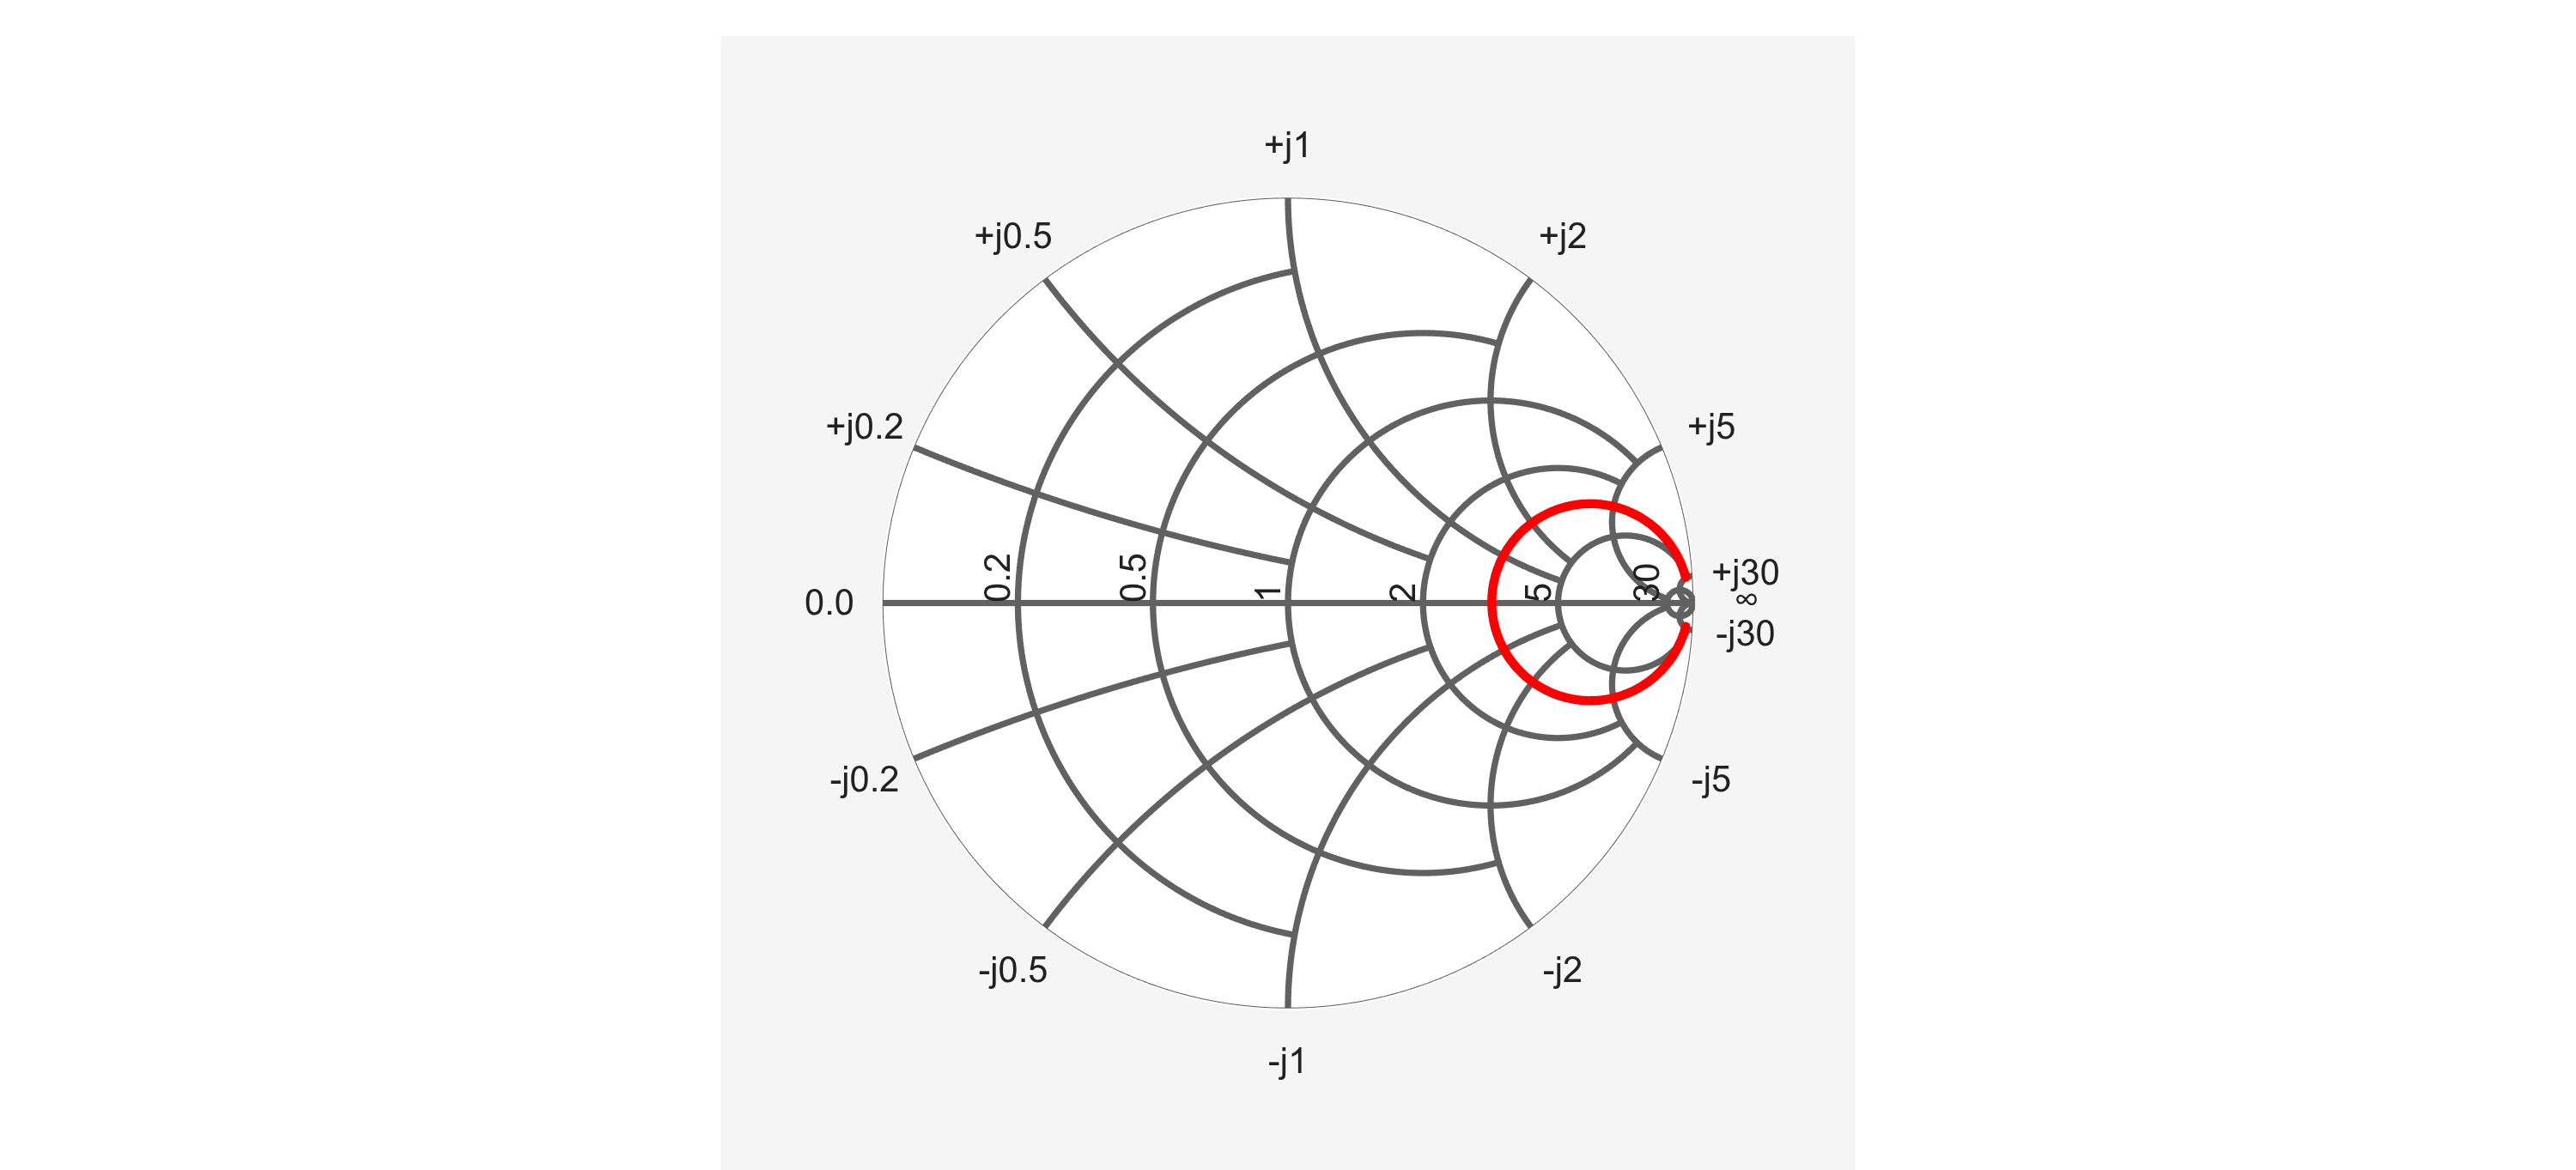
\includegraphics[width=0.6\textwidth]{./Images/Relazione5_Foto/2_1_c_smith_sfasato_open.png}
    \caption{Misura di $S_{11}$ sullo Smith chart con offset per portarlo in open position.}
\end{figure}
In seguito abbiamo introdotto un offset di 180° per portare il grafico in short position.
\begin{figure} [H]
    \centering
    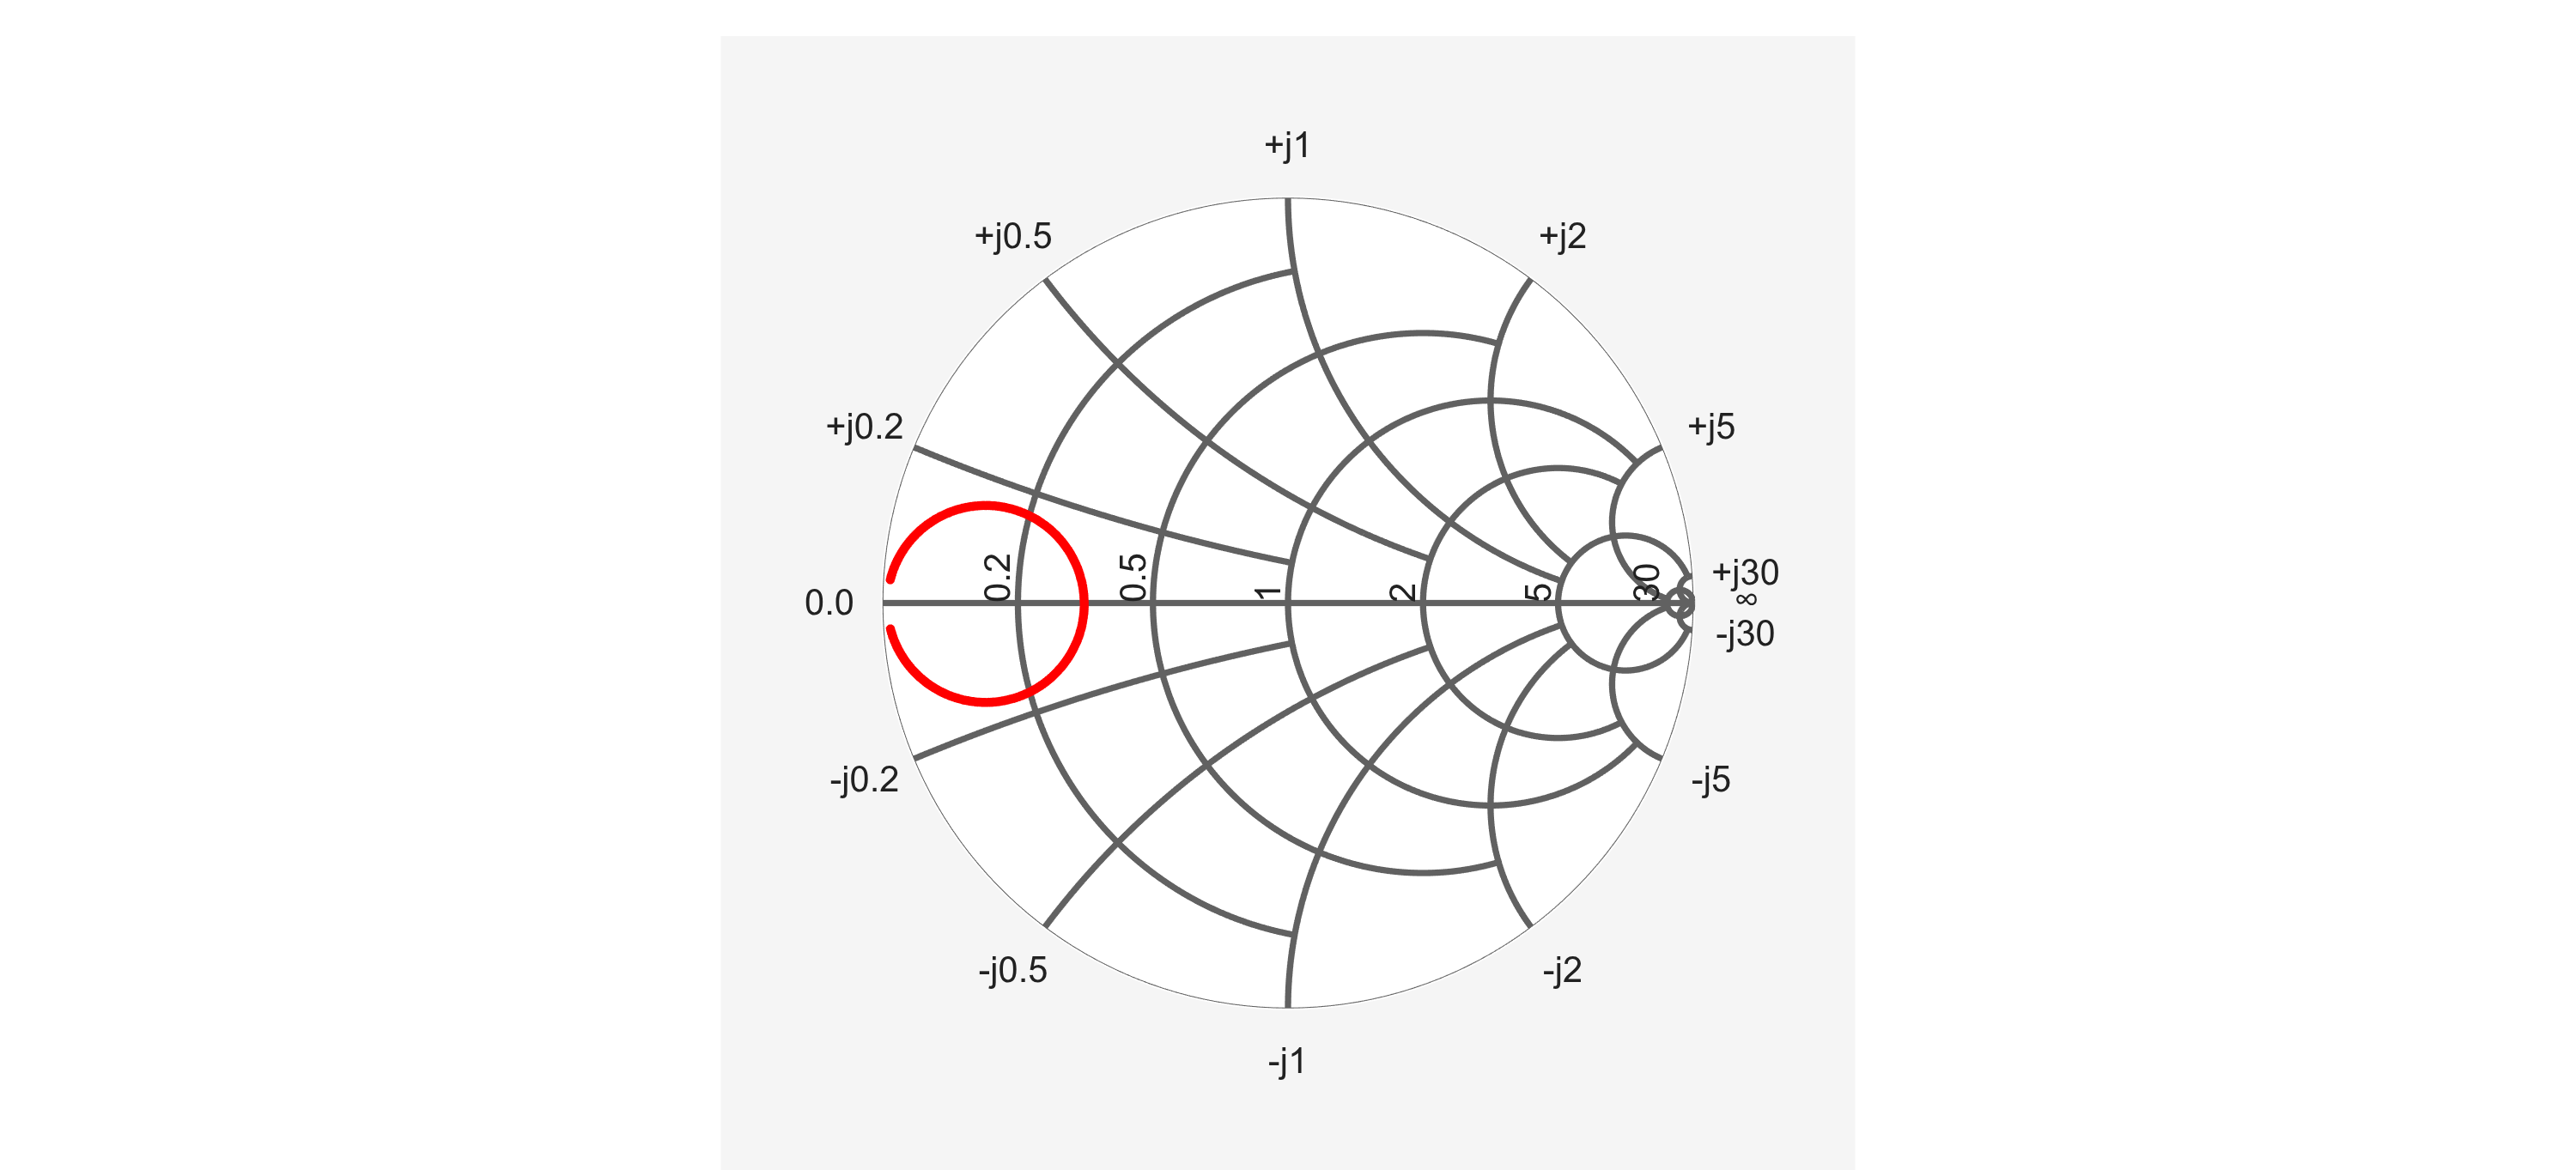
\includegraphics[width=0.6\textwidth]{./Images/Relazione5_Foto/2_1_d_short.png}
    \caption{Misura di $S_{11}$ sullo Smith chart con offset per portarlo in open position.}
\end{figure}
Fatti questi passaggi sullo Smith chart siamo passati a misurare il modulo dell'impedenza in dB al variare della frequenza.
\\I passaggi precedenti sono necesari per rendere valida la misura della banda dell'impedenza.
Il risultato è il seguente. 
\begin{figure}
    \centering
    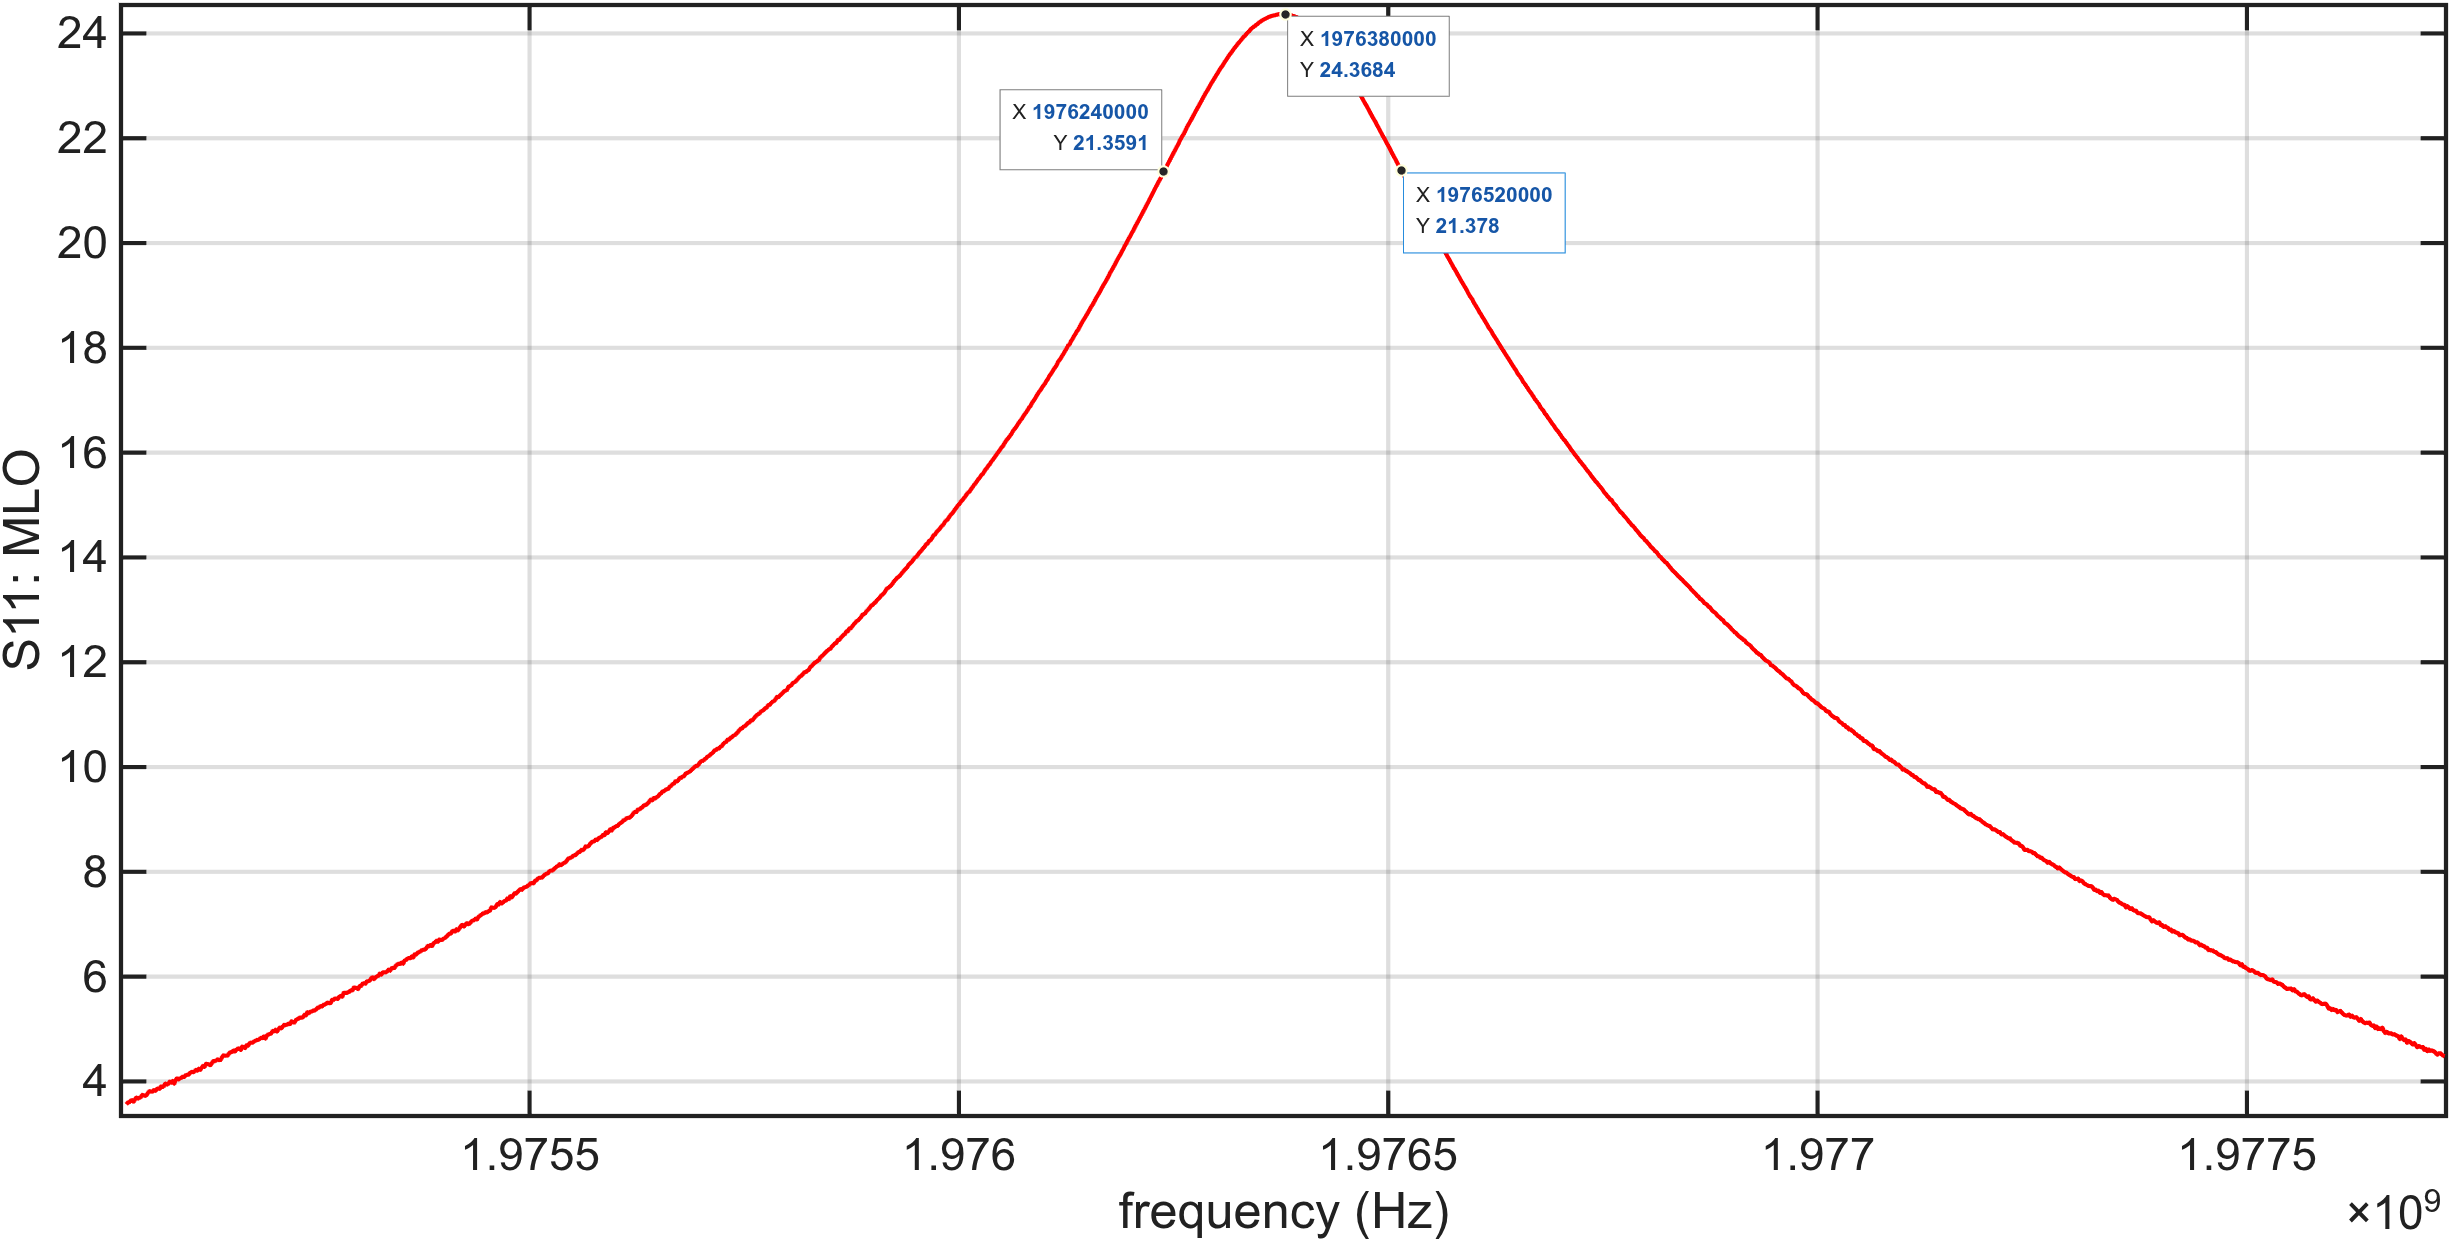
\includegraphics[width=0.4\textwidth]{./Images/Relazione5_Foto/2_1_e_impedenza_db.png}
    \caption{Misura dell'impedenza in dB e relativa banda a -3dB.}
\end{figure}
Dalla misura ricaviamo la banda, pari a 280KHz, da cui poi è facile ricavare $Q_0$:
\begin{equation}
    Q_0=\frac{f_0}{BW}=7.0585\cdot 10^3
\end{equation}


\subsection{Misura di $\beta$}
Dagli Smith chart del paragrafo precedente vediamo che l'origine non è inclusa, ciò vuol dire che $SWR(f_0)=\frac{1}{\beta}$.
\\Siamo quindi passati a graficare l'SWR:
\begin{figure}[H]
\centering
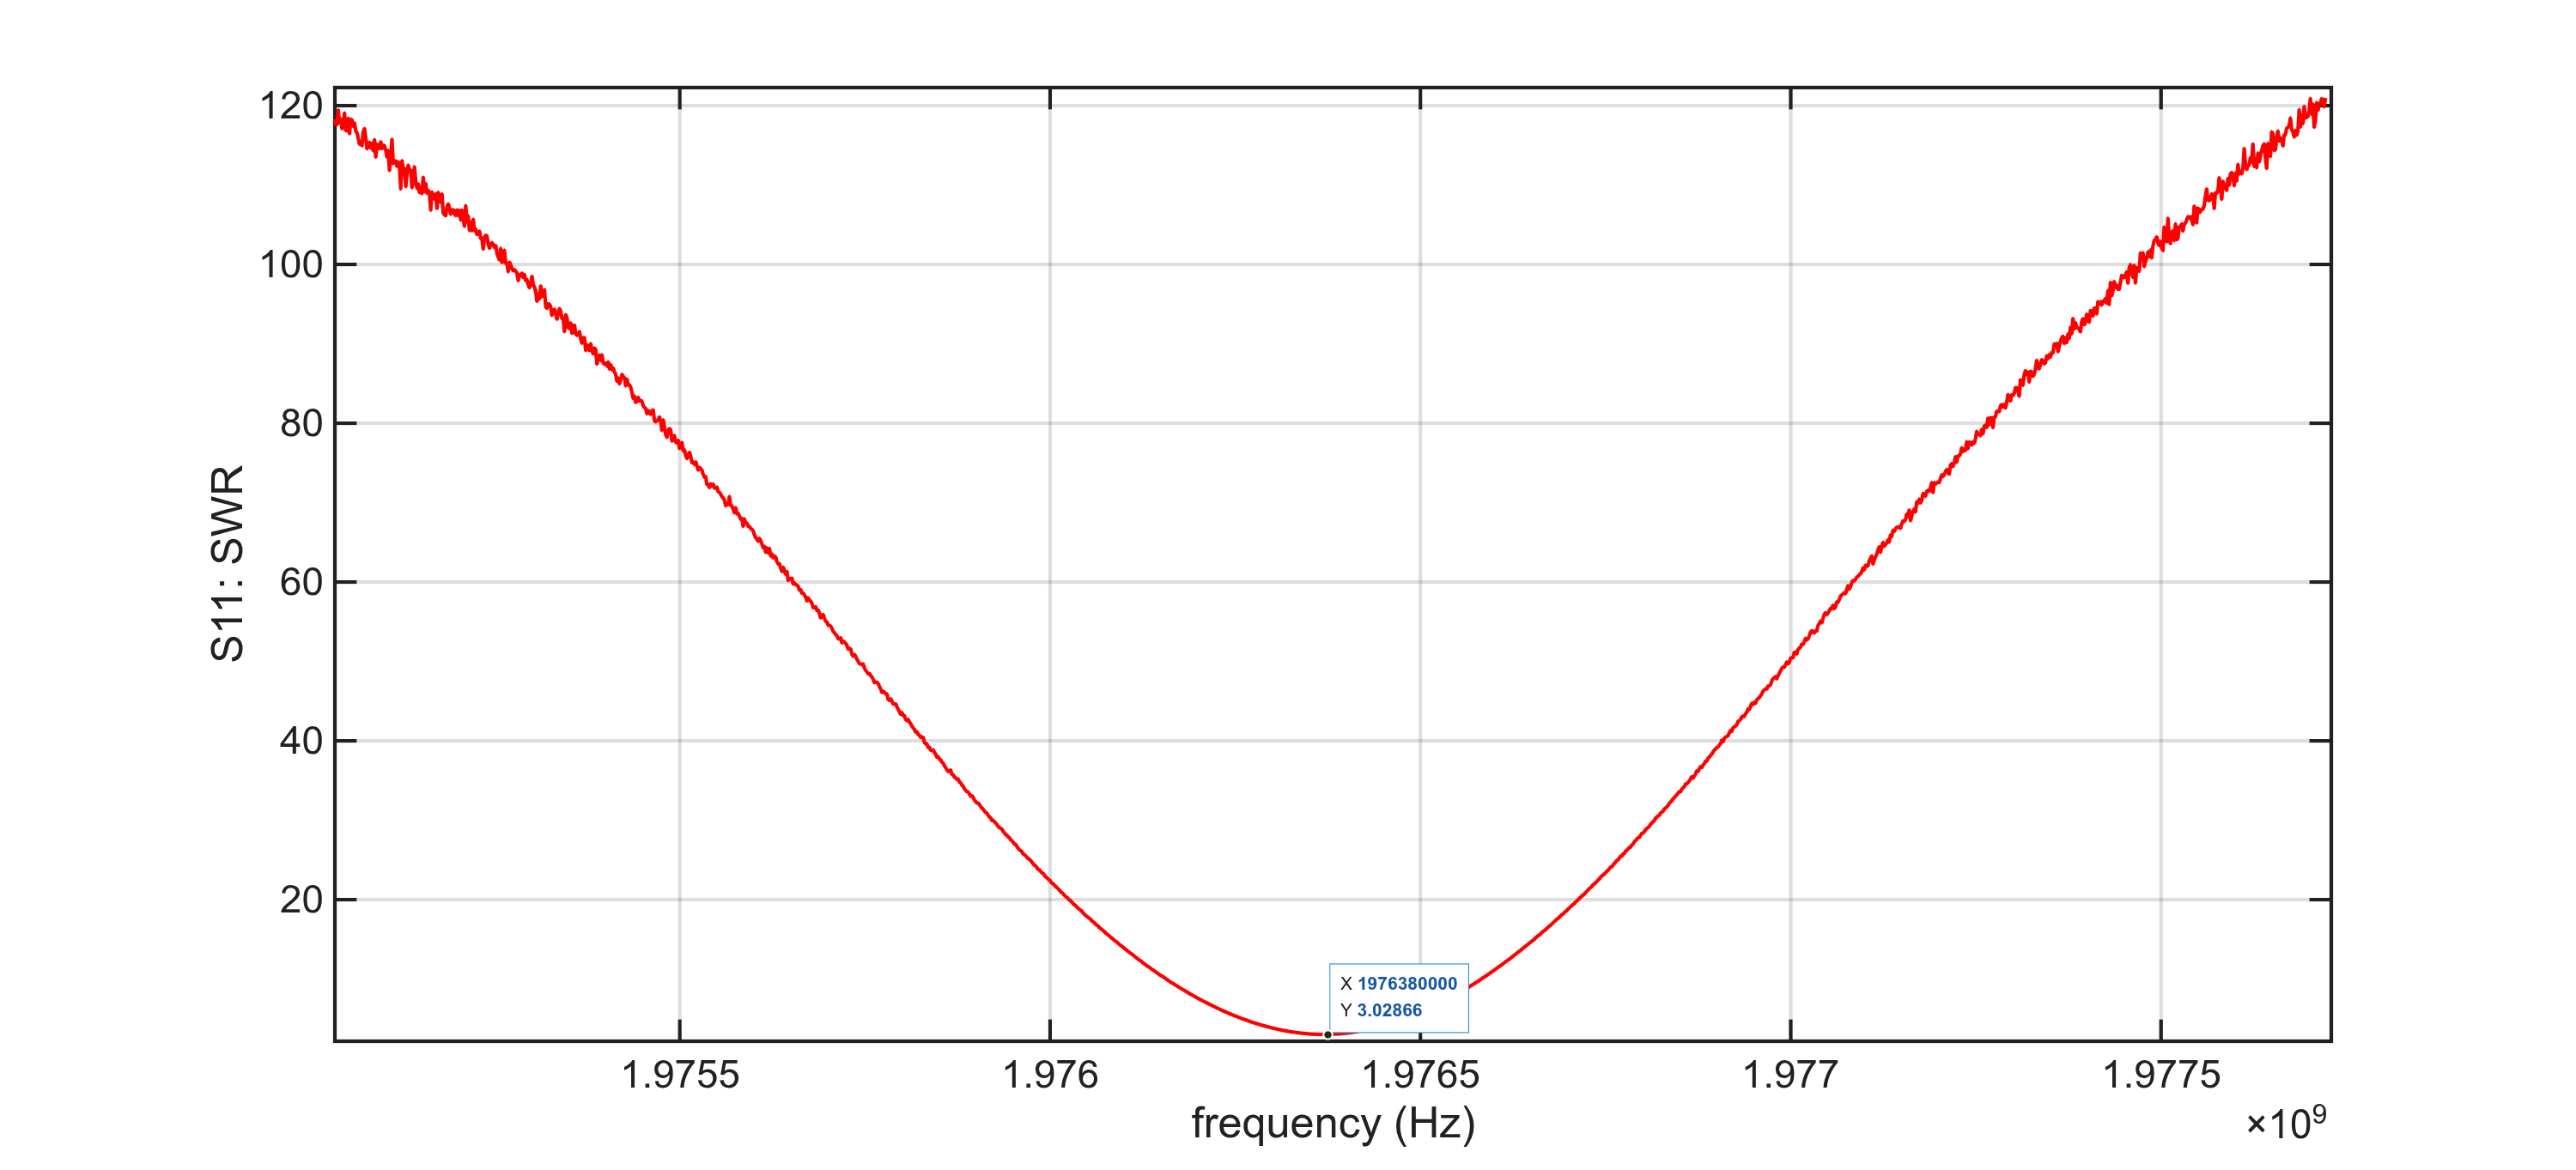
\includegraphics[width=0.8\textwidth]{./Images/Relazione5_Foto/2_1_f_SWR.png}    
\caption{Misura dello SWR.}
\end{figure}
Come si può vedere l'SWR vale 3.02866. Quindi:
\begin{equation}
    \beta=\frac{1}{SWR(f_0)}=0.3302
\end{equation}


\section{Stima di $Q_0$ dal linear fit della fase dell'impedenza}
Abbiamo valutato $Q_0$ dal linear fit della fase dell'impedenza. Essendo linear fit fatta per approssimare dei punti con una retta, abbiamo fatto il linear fit sono nella zona lineare della misura, e non per tutto 
lo span, in modo da avere una retta molto precisa nella zona lineare.      
\\Dal linear fit risulta:
\begin{figure}[H]
    \centering
    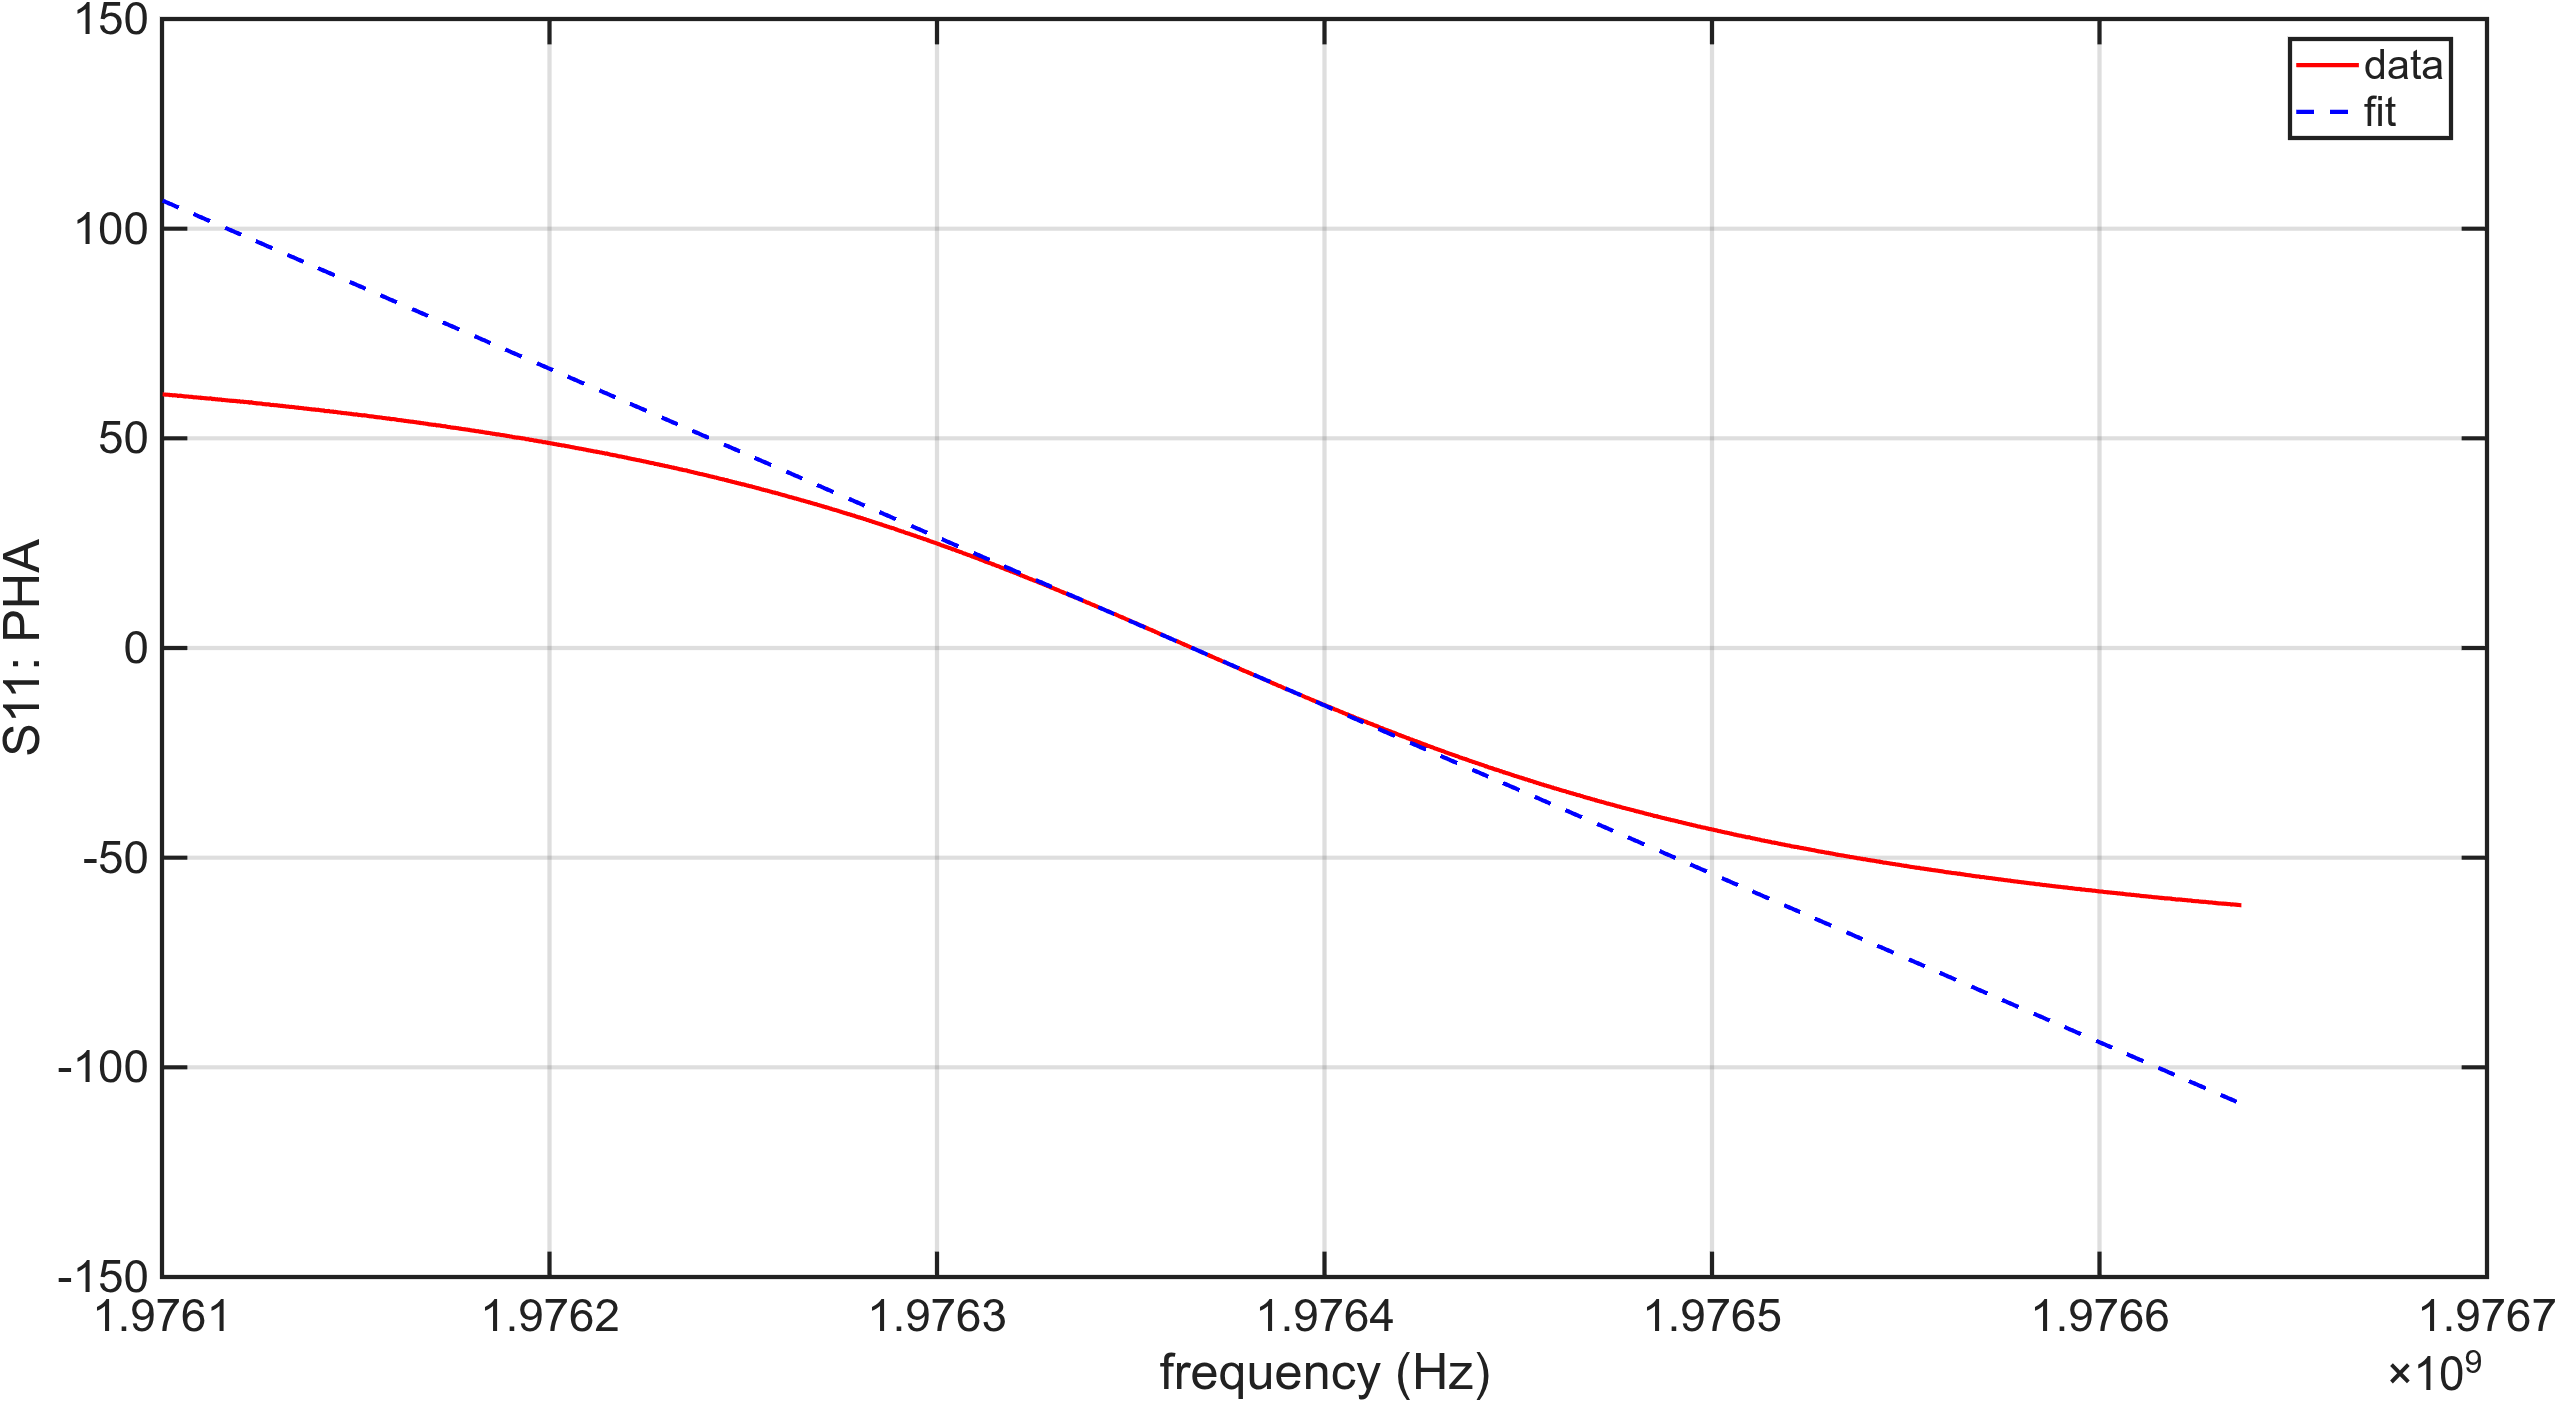
\includegraphics[width=0.6\textwidth]{./Images/Relazione5_Foto/2_2_fase_di_Z_con_linear_fit.png}
    \caption{Grafico della fase dell'impedenza con linear fit nella zona lineare.}
\end{figure}
Dal linearFit troviamo: $\overline{p}=-4.015318806635485\cdot 10^{-4}\,\mathrm{^\circ/Hz}$ e $\sigma_p=1.557248247795225\cdot10^{-7}\,\mathrm{^\circ/Hz}$



Con $\varphi$ in rad e $f$ in Hz, vicino alla risonanza:

\[
\varphi(f) \simeq -\frac{2Q_0}{f_0}(f-f_0)
\]

\[
\varphi(f)=p_{\mathrm{rad}}f+q
\]

\[
p_{\mathrm{rad}}=-\frac{2Q_0}{f_0}\quad[\mathrm{rad/Hz}]
\]

\[
Q_0=-\frac{p_{\mathrm{rad}}f_0}{2}
\]

La pendenza $p$ del fit è espressa in $\mathrm{^\circ/Hz}$, quindi $p_{\mathrm{rad}}=p\,\frac{\pi}{180}$ e:

\[
Q_0=-p\,\frac{\pi}{180}\,\frac{f_0}{2}
\]

Con \(f_0=1.976370\cdot10^9\,\mathrm{Hz}\):

\[
\overline{Q_0}=-\overline{p}\,\frac{\pi}{180}\,\frac{f_0}{2}
=4.015318806635485\cdot10^{-4}\,\mathrm{^\circ/Hz}\cdot\frac{\pi}{180}\,\mathrm{rad/^\circ}\cdot\frac{1.976370\cdot10^{9}\,\mathrm{Hz}}{2}
\simeq 6925.3
\]

\[
\sigma_{Q_0}=\sigma_p\,\frac{\pi}{180}\,\frac{f_0}{2}
=1.557248247795225\cdot10^{-7}\,\mathrm{^\circ/Hz}\cdot\frac{\pi}{180}\,\mathrm{rad/^\circ}\cdot\frac{1.976370\cdot10^{9}\,\mathrm{Hz}}{2}
\simeq 2.7
\]

\begin{equation}
Q_0=\overline{Q_0}\pm\sigma_{Q_0}=6925.3\pm2.7
\end{equation}

Il valore valutato con linearFit si discosta di circa 100 dal valore misuratro tramite l'impedenza.
\\L'errore, che comunque è piccolo, essendo circa del 1.4\%, è probabilmente dovuto all'approssimazione del linearFit, poichè la valutazione della pendenza rimane valida in un intorno stretto di $f_0$, ma muovendoci troppo nell'introno della frequenza di risonanza avremmo pochi campioni, quindi
siamo costretti ad espandere il numero di campioni e quindi la distanza da $f_0$. Inoltre anche il valore di $Q_0$ valutato con la pendenza della fase è un valore valutato tramite approssimazioni, e questa è un'altra
causa che ci porta a discostarci leggermente dal valore misurato nel punto precedente. 


\section{Confronto tra l'impedenza misurata e quella teorica}
Grafichiamo ora insieme la misurazione con il valore teorico sia per la fase che per il modulo dell'impedenza.
\begin{figure} [H]
    \centering
    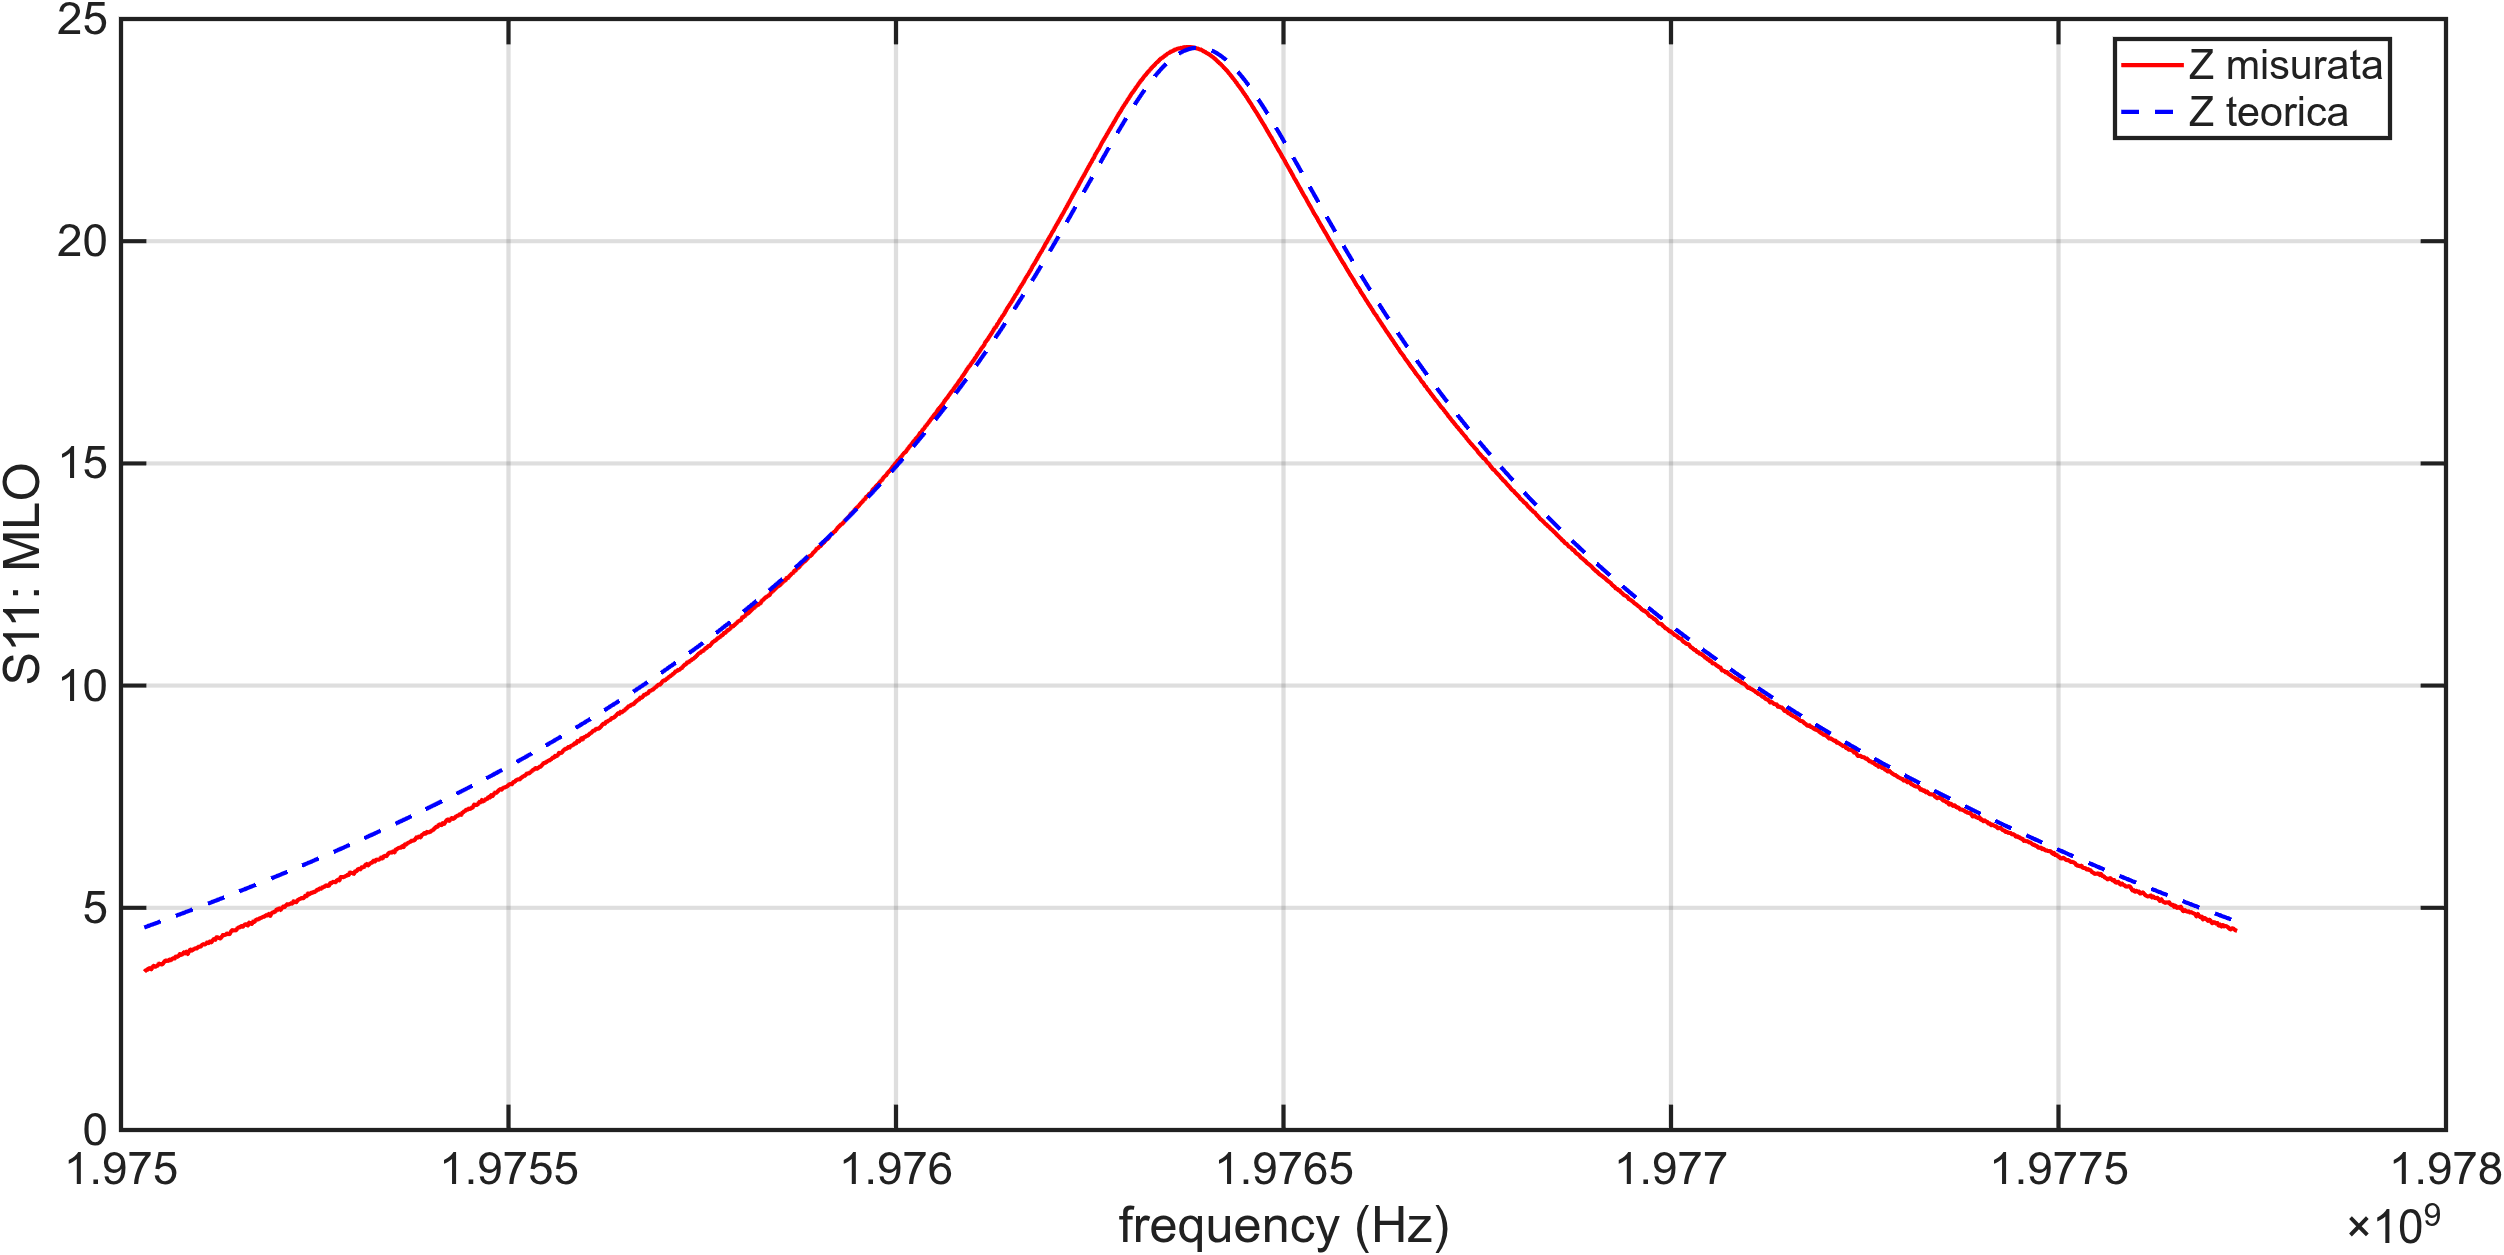
\includegraphics[width=0.8\textwidth]{./Images/Relazione5_Foto/2_2_Moduli_Z_misurato_e_teorico.png}
    \caption{Modulo dell'impedenza teorico e misurato.}
\end{figure}
\begin{figure} [H]
    \centering
    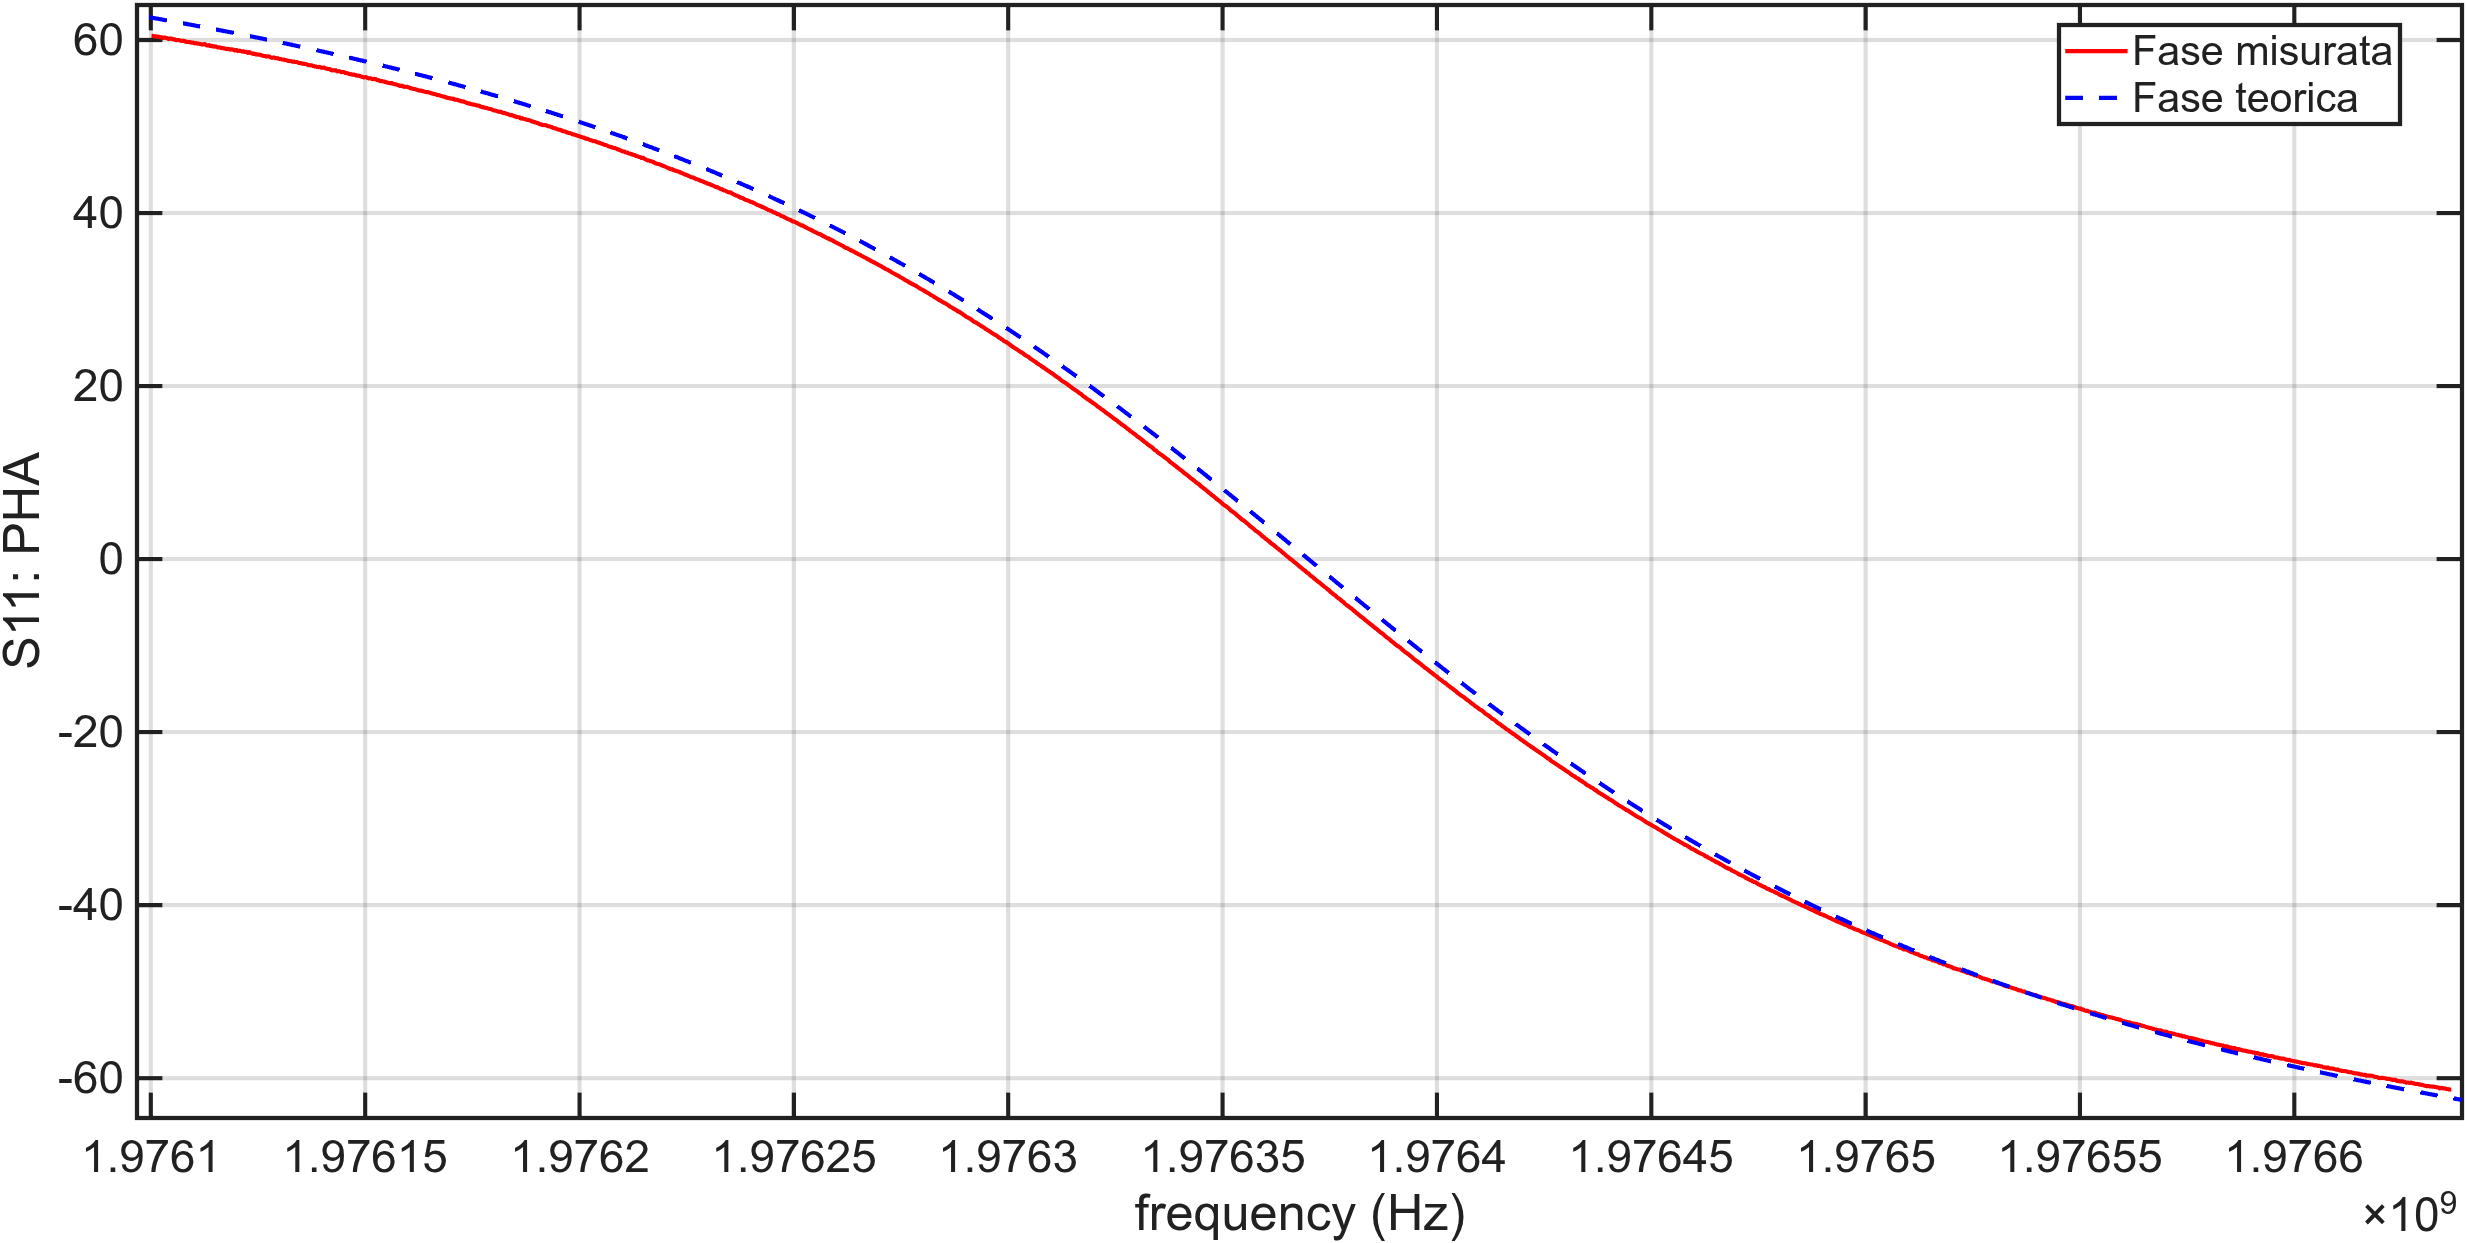
\includegraphics[width=0.8\textwidth]{./Images/Relazione5_Foto/2_2_Fasi_Z_teorico_e_misurato.png}
    \caption{Fase dell'impedenza teorica e misurata.}
\end{figure}
Come si può notare i grafici sia il modulo che la fase sono molto vicini tra loro. Possiamo quindi concludere che le misirazioni sono precise e valide.


\section{Confronto tra la misura di $|S_{11}|$ e il valore teorico}
Siamo passati poi a graficare il modulo di $S_{11}$ in dB e a confrontare il valore misurato
con quello teorico dalle formule.
Ricordiamo le formule teoriche:
\begin{equation*}
    S_{11t} = \sqrt{\frac{(\beta-1)^2 + (Q_0 \cdot \delta)^2}{(\beta+1)^2 + (Q_0 \cdot \delta)^2}}
\end{equation*}
\begin{equation*}
    \delta = \frac{f}{f_0} - \frac{f_0}{f}
\end{equation*}
Il risultato è il seguente.
\begin{figure}[H]
    \centering
    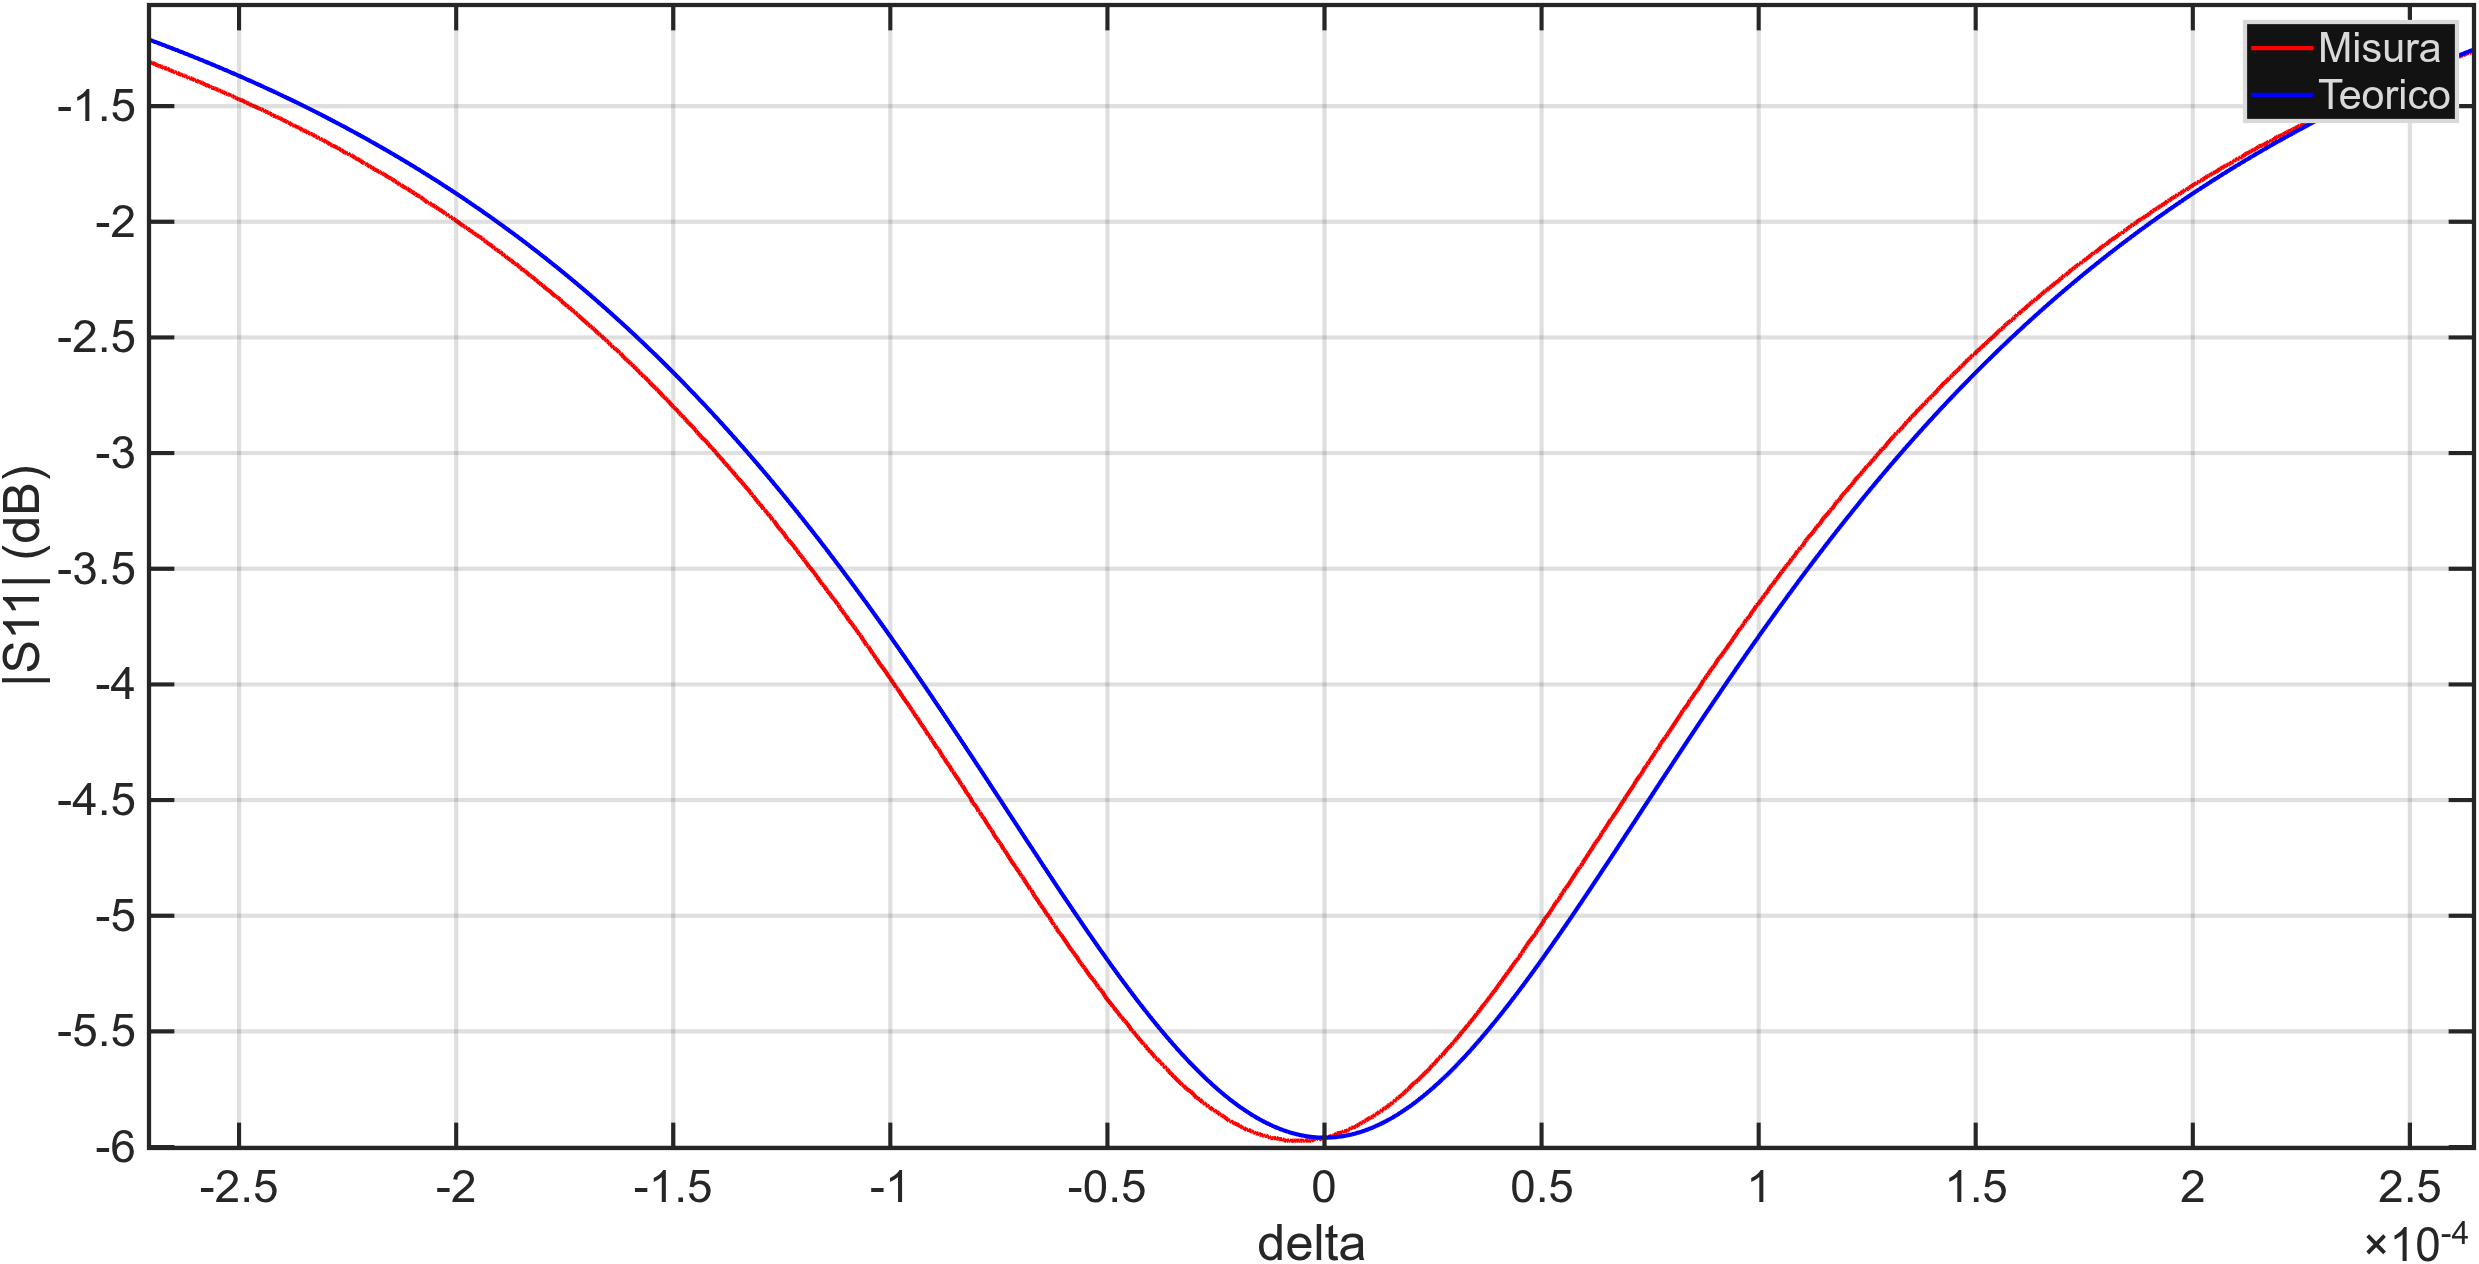
\includegraphics[width=0.8\textwidth]{./Images/Relazione5_Foto/2_4_S11_modulo_teorico_e_misurato.png}
    \caption{Confrotno di $|S_{11}|_{dB}$ misurato e teorico rispetto a $\delta$.}
\end{figure}
I due grafici sono molto simili, quindi possiamo concludere che la misurazione è valida.

\section{Misura di $Q_0$ dalla pendenza della fase}


\chapter{Deflettore RF (banda S): modi di tipo TM$_{110}$}

\chapter{Deflettore RF (banda S): modi di tipo TM$_{010}$ e TM$_{110}$}

\chapter{Cavità multicella decelerante (banda X)}


\end{document}
